\documentclass[11pt]{article}

% The four macros of the header standard; tools/zenodo/publish_revision.py patches them when it reserves the DOI.
\newcommand{\doctype}{Preprint}
\newcommand{\docversion}{v1.00.000}
\newcommand{\docdate}{4 November 2026}
\newcommand{\versiondoi}{10.5281/zenodo.0}
\newcommand{\conceptdoi}{10.5281/zenodo.0}
\newcommand{\docidentity}{CAOS\_Contraste, the validation of the risk models of a bank}

% The packages and conventions every Contraste manuscript shares (CAOS_MANAGE conventions/manuscript-content-bar.md
% section 2). A document sets its class, the four header macros and \docidentity, then % The packages and conventions every Contraste manuscript shares (CAOS_MANAGE conventions/manuscript-content-bar.md
% section 2). A document sets its class, the four header macros and \docidentity, then % The packages and conventions every Contraste manuscript shares (CAOS_MANAGE conventions/manuscript-content-bar.md
% section 2). A document sets its class, the four header macros and \docidentity, then \input{../_shared/preamble}.
\usepackage[T1]{fontenc}
\usepackage[utf8]{inputenc}
\usepackage{lmodern}
\usepackage{microtype}
\usepackage[a4paper,margin=2.5cm]{geometry}
\usepackage{amsmath,amssymb,amsthm,mathtools,bm}
\usepackage{graphicx}
\usepackage{booktabs,longtable,tabularx,array,multirow}
\usepackage{siunitx}
\usepackage{algorithm}
\usepackage{algpseudocode}
\usepackage{caption,subcaption}
\usepackage{xcolor}
\usepackage[numbers,sort&compress]{natbib}
\usepackage[hidelinks]{hyperref}
\usepackage{cleveref}
\usepackage{orcidlink}

\sisetup{group-separator={,},group-minimum-digits=4,detect-all}
\graphicspath{{figures/}{../figures/}}
\captionsetup{font=small,labelfont=bf}
\setlength{\LTcapwidth}{\textwidth}

% Theorem environments for the Theory sections of the manuscripts.
\newtheorem{proposition}{Proposition}
\newtheorem{lemma}{Lemma}
\newtheorem{corollary}{Corollary}
\theoremstyle{definition}
\newtheorem{definition}{Definition}
\newtheorem{assumption}{Assumption}
\theoremstyle{remark}
\newtheorem{remark}{Remark}

% Notation shared by the documents (each defines it again in its notation table).
\newcommand{\E}{\mathbb{E}}
\newcommand{\Prob}{\mathbb{P}}
\newcommand{\Var}{\operatorname{Var}}
\newcommand{\Cov}{\operatorname{Cov}}
\newcommand{\VaR}{\operatorname{VaR}}
\newcommand{\ES}{\operatorname{ES}}
\newcommand{\PD}{\mathrm{PD}}
\newcommand{\LGD}{\mathrm{LGD}}
\newcommand{\EAD}{\mathrm{EAD}}
\newcommand{\ECL}{\mathrm{ECL}}
\newcommand{\indic}{\mathbf{1}}
\newcommand{\R}{\mathbb{R}}
\newcommand{\dd}{\,\mathrm{d}}

% The page-1 header block (CAOS_MANAGE conventions/manuscript-header-standard.md). The document defines \doctype,
% \docversion, \docdate, \versiondoi, \conceptdoi and \docidentity before this file; the publishing tool patches the four
% macros of the standard when it reserves the version DOI.
\newcommand{\docrepo}{github.com/fsantibanezleal/CAOS\_Contraste}
\newcommand{\headerblock}{%
\begin{center}
\fbox{\parbox{0.94\textwidth}{\small\raggedright
\textbf{\doctype} \quad$\cdot$\quad \docversion, \docdate \quad$\cdot$\quad Licence CC BY 4.0\\[2pt]
CAOS open-research programme \quad$\cdot$\quad \docidentity\\[2pt]
Version DOI \href{https://doi.org/\versiondoi}{\texttt{\versiondoi}} \quad$\cdot$\quad
concept DOI (always latest) \href{https://doi.org/\conceptdoi}{\texttt{\conceptdoi}}\\[2pt]
Not peer reviewed. Source code, data and computational records: \href{https://\docrepo}{\texttt{\docrepo}}
}}
\end{center}
\vspace{4pt}}
.
\usepackage[T1]{fontenc}
\usepackage[utf8]{inputenc}
\usepackage{lmodern}
\usepackage{microtype}
\usepackage[a4paper,margin=2.5cm]{geometry}
\usepackage{amsmath,amssymb,amsthm,mathtools,bm}
\usepackage{graphicx}
\usepackage{booktabs,longtable,tabularx,array,multirow}
\usepackage{siunitx}
\usepackage{algorithm}
\usepackage{algpseudocode}
\usepackage{caption,subcaption}
\usepackage{xcolor}
\usepackage[numbers,sort&compress]{natbib}
\usepackage[hidelinks]{hyperref}
\usepackage{cleveref}
\usepackage{orcidlink}

\sisetup{group-separator={,},group-minimum-digits=4,detect-all}
\graphicspath{{figures/}{../figures/}}
\captionsetup{font=small,labelfont=bf}
\setlength{\LTcapwidth}{\textwidth}

% Theorem environments for the Theory sections of the manuscripts.
\newtheorem{proposition}{Proposition}
\newtheorem{lemma}{Lemma}
\newtheorem{corollary}{Corollary}
\theoremstyle{definition}
\newtheorem{definition}{Definition}
\newtheorem{assumption}{Assumption}
\theoremstyle{remark}
\newtheorem{remark}{Remark}

% Notation shared by the documents (each defines it again in its notation table).
\newcommand{\E}{\mathbb{E}}
\newcommand{\Prob}{\mathbb{P}}
\newcommand{\Var}{\operatorname{Var}}
\newcommand{\Cov}{\operatorname{Cov}}
\newcommand{\VaR}{\operatorname{VaR}}
\newcommand{\ES}{\operatorname{ES}}
\newcommand{\PD}{\mathrm{PD}}
\newcommand{\LGD}{\mathrm{LGD}}
\newcommand{\EAD}{\mathrm{EAD}}
\newcommand{\ECL}{\mathrm{ECL}}
\newcommand{\indic}{\mathbf{1}}
\newcommand{\R}{\mathbb{R}}
\newcommand{\dd}{\,\mathrm{d}}

% The page-1 header block (CAOS_MANAGE conventions/manuscript-header-standard.md). The document defines \doctype,
% \docversion, \docdate, \versiondoi, \conceptdoi and \docidentity before this file; the publishing tool patches the four
% macros of the standard when it reserves the version DOI.
\newcommand{\docrepo}{github.com/fsantibanezleal/CAOS\_Contraste}
\newcommand{\headerblock}{%
\begin{center}
\fbox{\parbox{0.94\textwidth}{\small\raggedright
\textbf{\doctype} \quad$\cdot$\quad \docversion, \docdate \quad$\cdot$\quad Licence CC BY 4.0\\[2pt]
CAOS open-research programme \quad$\cdot$\quad \docidentity\\[2pt]
Version DOI \href{https://doi.org/\versiondoi}{\texttt{\versiondoi}} \quad$\cdot$\quad
concept DOI (always latest) \href{https://doi.org/\conceptdoi}{\texttt{\conceptdoi}}\\[2pt]
Not peer reviewed. Source code, data and computational records: \href{https://\docrepo}{\texttt{\docrepo}}
}}
\end{center}
\vspace{4pt}}
.
\usepackage[T1]{fontenc}
\usepackage[utf8]{inputenc}
\usepackage{lmodern}
\usepackage{microtype}
\usepackage[a4paper,margin=2.5cm]{geometry}
\usepackage{amsmath,amssymb,amsthm,mathtools,bm}
\usepackage{graphicx}
\usepackage{booktabs,longtable,tabularx,array,multirow}
\usepackage{siunitx}
\usepackage{algorithm}
\usepackage{algpseudocode}
\usepackage{caption,subcaption}
\usepackage{xcolor}
\usepackage[numbers,sort&compress]{natbib}
\usepackage[hidelinks]{hyperref}
\usepackage{cleveref}
\usepackage{orcidlink}

\sisetup{group-separator={,},group-minimum-digits=4,detect-all}
\graphicspath{{figures/}{../figures/}}
\captionsetup{font=small,labelfont=bf}
\setlength{\LTcapwidth}{\textwidth}

% Theorem environments for the Theory sections of the manuscripts.
\newtheorem{proposition}{Proposition}
\newtheorem{lemma}{Lemma}
\newtheorem{corollary}{Corollary}
\theoremstyle{definition}
\newtheorem{definition}{Definition}
\newtheorem{assumption}{Assumption}
\theoremstyle{remark}
\newtheorem{remark}{Remark}

% Notation shared by the documents (each defines it again in its notation table).
\newcommand{\E}{\mathbb{E}}
\newcommand{\Prob}{\mathbb{P}}
\newcommand{\Var}{\operatorname{Var}}
\newcommand{\Cov}{\operatorname{Cov}}
\newcommand{\VaR}{\operatorname{VaR}}
\newcommand{\ES}{\operatorname{ES}}
\newcommand{\PD}{\mathrm{PD}}
\newcommand{\LGD}{\mathrm{LGD}}
\newcommand{\EAD}{\mathrm{EAD}}
\newcommand{\ECL}{\mathrm{ECL}}
\newcommand{\indic}{\mathbf{1}}
\newcommand{\R}{\mathbb{R}}
\newcommand{\dd}{\,\mathrm{d}}

% The page-1 header block (CAOS_MANAGE conventions/manuscript-header-standard.md). The document defines \doctype,
% \docversion, \docdate, \versiondoi, \conceptdoi and \docidentity before this file; the publishing tool patches the four
% macros of the standard when it reserves the version DOI.
\newcommand{\docrepo}{github.com/fsantibanezleal/CAOS\_Contraste}
\newcommand{\headerblock}{%
\begin{center}
\fbox{\parbox{0.94\textwidth}{\small\raggedright
\textbf{\doctype} \quad$\cdot$\quad \docversion, \docdate \quad$\cdot$\quad Licence CC BY 4.0\\[2pt]
CAOS open-research programme \quad$\cdot$\quad \docidentity\\[2pt]
Version DOI \href{https://doi.org/\versiondoi}{\texttt{\versiondoi}} \quad$\cdot$\quad
concept DOI (always latest) \href{https://doi.org/\conceptdoi}{\texttt{\conceptdoi}}\\[2pt]
Not peer reviewed. Source code, data and computational records: \href{https://\docrepo}{\texttt{\docrepo}}
}}
\end{center}
\vspace{4pt}}

\setlength{\emergencystretch}{3em}

\newcommand{\HPL}{\mathrm{HPL}}
\newcommand{\RTPL}{\mathrm{RTPL}}
\newcommand{\sgn}{\operatorname{sgn}}

\title{A scale-and-level complement to the FRTB profit and loss attribution test}
\author{Felipe Santib\'a\~nez-Leal~\orcidlink{0000-0002-0150-3246}\\
\small CAOS open-research programme, Santiago, Chile\\
\small \texttt{fsantibanez@gmail.com}}
\date{\docdate}

\begin{document}
\maketitle
\headerblock

\begin{abstract}
The profit and loss attribution test of the Basel market risk standard compares the hypothetical and the risk-theoretical profit and loss of a trading desk through a Spearman correlation of the levels and a Kolmogorov--Smirnov distance, and its zones sit at thresholds that a desk with a faulty model can pass.
On a generator of desk profit and loss with a known true risk model, a model fed a volatility twenty days old is flagged by neither statistic in any of 1,000 replications.
We propose a complement added beside the regulatory zone: a Mincer--Zarnowitz regression of the hypothetical on the risk-theoretical profit and loss with a joint Wald test of intercept zero and slope one under an HC3 covariance, the Spearman correlation of the absolute values, and the Spearman correlation of their 20-day rolling means, each with a critical value read from a simulated null so that the false-alarm rate is stated.
At a family size of 1\% the complement flags the stale-volatility model in 99.9\% of 1,000 replications (95\% Wilson interval 99.4 to 100.0\%) with a held-out false-alarm rate of 0.9\% (0.5 to 1.7\%), where the regulatory zone flags 0.0\%.
Against published comparators run on the same desk-years, the rolling-mean statistic has the largest area under the ROC curve at lags of 5, 10 and 20 days.
The stated size does not transfer to desks whose volatility is more persistent or more dispersed (4.0\% and 6.2\%) or whose pricing noise is larger (99.0\%), so the thresholds have to be calibrated on each desk's own null.
The complement does not replace the regulatory zone: it is weak against a one-day misalignment and against a wrong correlation.
\end{abstract}

\section{Introduction}
\label{sec:introduction}

A bank that wants to measure the market risk of a trading desk with its own internal model, instead of the standardised formula, has to show under the revised Basel market risk standard that the model describes the desk it is meant to describe.
The standard \citep{bcbs2019}, first published in January 2016 \citep{bcbs2016} and revised in January 2019, asks for two tests at the level of the desk.
The first is a back-test of the desk's value-at-risk against its realised profit and loss.
The second is the profit and loss attribution test, which compares, over the most recent 250 trading days, the hypothetical profit and loss of the desk (HPL, the revaluation of the positions held at the close of the previous day by the front-office pricing models) with the risk-theoretical profit and loss (RTPL, the revaluation of the same positions by the risk model, with the same market moves).
A desk whose risk model reproduces the pricing model closely is eligible for the internal model; a desk in the red zone is not, and a desk in the amber zone carries a capital surcharge.
The comparison is made with two numbers: the Spearman correlation of the daily levels of HPL and RTPL \citep{spearman1904} and the two-sample Kolmogorov--Smirnov distance between their empirical distributions \citep{smirnov1948}.

Both numbers are blind to the timing of the scale of the profit and loss.
A rank correlation of levels is dominated by the sign and the order of the daily moves, which the two series share whenever the risk model has the right factors and the right sensitivities; a Kolmogorov--Smirnov distance compares two distributions accumulated over a year, in which a volatility that moves late and a volatility that moves on time have the same marginal law.
A risk model that feeds yesterday's positions and today's factor moves into a volatility estimate that is several weeks old therefore passes both statistics while it understates the risk in every rising-volatility episode and overstates it in every falling one.
We make this concrete on a generator of desk profit and loss whose true risk model is known (the C13 case of the validation product described in Section~\ref{sec:experimental-design}): with a volatility input twenty days old, none of 1,000 replications leaves the green zone, whereas the planted deficiency changes the correlation of the 20-day rolling means of the absolute profit and loss of the two series from 0.99 to 0.69 on average.

The gap this paper addresses is therefore not the construction of a new regulatory test but the absence, beside the regulatory one, of a statistic of the scale of the profit and loss and of its timing, with a false-alarm rate that is stated rather than inherited from thresholds written for other purposes.
The published literature has the ingredients separately: the regression of realisations on forecasts with a joint test of intercept zero and slope one \citep{mincer1969}, the evaluation of volatility forecasts through proxies \citep{patton2011,patton2009}, the heteroskedasticity-consistent covariance \citep{white1980,mackinnon1985}, and critical values read from simulated draws of the null \citep{dufour2006}.
None of the works we found combines them into a complement to the attribution test of the market risk standard, and none of them measures what such a complement flags on desks with a known planted deficiency.

We propose the complement in Section~\ref{sec:proposed-method}.
It is made of three statistics computed on the same 250-day pair as the regulatory test: the Wald statistic of the joint hypothesis that the regression of HPL on RTPL has intercept zero and slope one, under an HC3 covariance; the Spearman correlation of the absolute values of HPL and RTPL; and the Spearman correlation of their 20-day rolling means.
Each statistic is compared with a critical value read from the empirical distribution of the same statistic on simulated desk-years of a model with nothing planted, so that the decision has a stated false-alarm rate, and the three decisions are combined with a Bonferroni split so that their union has a stated rate as well.
The complement is added beside the regulatory zone and returns it unchanged; it has no regulatory standing.

The contributions are the following.
\begin{enumerate}
\item The complement itself, specified in full with its calibration rule, its algorithm and its implementation in the open-source engine \texttt{riskvalidation} 1.1.0.
\item Four propositions with proofs: the exact out-of-sample false-alarm rate of a critical value read from $N$ simulated null values; the population slope of the regression of HPL on RTPL when the volatility input of the risk model is $L$ days old, which explains why a Wald test is weak against that deficiency; a closed form for the correlation of the rolling means of the absolute series, which explains why the rolling-mean statistic is strong; and the invariance of the rank statistics under rescaling, which assigns a different defect to each component.
\item An evaluation on 6,000 committed desk-years, on 30,000 further desk-years from five independent bakes, on a ladder of volatility lags from 2 to 80 days, on six desks whose generator differs from the calibration null and on six constant mis-scales and level errors, in which nine published or regulatory detectors are run on the same series as the proposed ones.
\item An ablation of every component, of the rolling window, of the covariance and of the multiplicity correction.
\item Negative results: the Wald component does not see a missing basis (0.9\%) or a stale volatility (14.2\%); the rolling statistic alone does not see a wrong correlation (4.5\%) and is weak against a one-day misalignment (42.3\%), which the union flags only through the Wald statistic; and the stated size does not transfer to desks whose volatility law differs from the calibration null.
\end{enumerate}

The main result is that, at a family size of 1\%, the complement flags the stale-volatility desk in 99.9\% of 1,000 replications against 0.0\% for the regulatory zone, with a held-out false-alarm rate of 0.9\%, and that a Spearman correlation of the levels whose threshold is merely recalibrated to the same 1\% size flags the same desk in 55.2\% of replications, which locates much of the regulatory blind spot in the thresholds of the zone and the rest in the choice of statistic.
Section~\ref{sec:related-work} places the work among the published methods, Section~\ref{sec:problem} states the problem, Section~\ref{sec:proposed-method} the method, Section~\ref{sec:theory} the theory, Section~\ref{sec:experimental-design} the design of the experiments, Sections~\ref{sec:results} and~\ref{sec:ablation} the results and the ablation, and Sections~\ref{sec:discussion} to~\ref{sec:conclusions} the discussion, the limits, the reproduction and the conclusions.

\section{Related work}
\label{sec:related-work}

The complement sits between three bodies of work: the regulatory attribution test and its two statistics, the econometric evaluation of forecasts of a level and of a volatility, and the statistical machinery needed to give a decision a stated false-alarm rate.
This section groups the published methods by approach, says what each assumes, gives and misses with respect to the problem of Section~\ref{sec:problem}, and states where the proposed method stands.

\subsection{The regulatory attribution test and its statistics}
\label{sec:rw-regulatory}

The market risk standard of the Basel Committee \citep{bcbs2019,bcbs2016} compares the hypothetical and the risk-theoretical profit and loss of a desk over 250 trading days with two statistics and sorts the desk into a green, amber or red zone from fixed thresholds on each.
The Spearman correlation \citep{spearman1904} is the Pearson correlation of the ranks; it is unchanged by any increasing transformation of either series, so it assumes that the order of the daily moves is what matters, gives a measure of monotone association and fails whenever two series share their order while differing in the size or the timing of their scale.
The Kolmogorov--Smirnov distance \citep{smirnov1948} is the largest vertical gap between the two empirical distribution functions; it assumes exchangeability of the days inside each series, gives a measure of the marginal difference and fails whenever two series have the same marginal law and a different dynamics, which is the case of a volatility that moves late.
Neither statistic has a stated false-alarm rate on a desk-year of a correct model: the zone thresholds are fixed numbers, and we measure in Section~\ref{sec:results} that on the C13 generator the correct model never leaves the green zone while the distance between the statistic of a correct model and the threshold is large (a mean Spearman correlation of 0.992 against a green limit of 0.80, a mean distance of 0.033 against 0.09).
The proposed method stays in this family of two-series statistics computed on the same 250-day pair and adds what the family does not contain, a statistic of scale and of its timing, with a calibrated threshold.

\subsection{Evaluation of forecasts by regression and by proxies}
\label{sec:rw-forecast}

The regression of realisations on forecasts, with a joint test of intercept zero and slope one, is due to \citet{mincer1969}: a forecast is efficient in the sense of being unbiased and of using its information fully when the realisation has conditional mean equal to the forecast.
The regression assumes a forecast of a conditional mean and a realisation observed with noise that is uncorrelated with the forecast, gives a test of level and scale, and fails against any defect that leaves the conditional mean intact.
\citet{patton2009} survey the use of the regression for forecasts of volatility and correlation, with squared or absolute returns as proxies for the unobserved volatility, and \citet{patton2011} proves that only a family of loss functions ranks volatility forecasts consistently when the true volatility is replaced by a noisy proxy; \citet{andersen1998} show that a high-frequency realised volatility makes the proxy much less noisy than a squared daily return.
The comparison of competing forecasts has a literature of its own: the test of equal predictive accuracy of \citet{diebold1995}, its conditional version \citep{giacomini2006}, the model confidence set \citep{hansen2011}, the study of whether any volatility model beats a GARCH(1,1) \citep{hansen2005}, and the theory of consistent scoring functions for point forecasts \citep{gneiting2011}.
These tests compare forecasts with a realisation or with each other; the attribution problem has no external realisation, since both series are model outputs on the same market moves, and the quantity of interest is the agreement of two series rather than the accuracy of one.
The proposed method borrows the regression and the absolute-value proxy and applies them to the pair of series of the attribution test, with a rank correlation of rolling means that is built for the scale-timing defect the regression does not see.

\subsection{Back-testing of risk measures}
\label{sec:rw-backtest}

The proportion-of-failures test of \citet{kupiec1995} checks that a value-at-risk is exceeded at its nominal rate; \citet{christoffersen1998} adds a likelihood-ratio test of independence of the exceedances and a joint test of conditional coverage; \citet{berkowitz2001} and \citet{diebold1998} test the whole predictive density through the probability integral transform of the realisations; \citet{engle2004} model the quantile directly by regression and test its dynamics; \citet{fissler2016} show that value-at-risk and expected shortfall are jointly elicitable, which allows a joint scoring function.
Back-tests assume a realised loss series and a risk measure forecast for each day, give a decision about the risk measure and have little power with 250 days at a 99\% level, where about two and a half exceedances are expected.
The regulation applies a back-test at the desk level next to the attribution test, and we run the desk limit of the standard and the conditional-coverage test of \citet{christoffersen1998} on the same desk-years in Section~\ref{sec:results}; both are weak against a stale volatility (0.5\% and 12.7\%).
The proposed method is not a back-test: it needs no risk measure, only the two profit and loss series, and it asks whether the risk model's scale tracks the pricing model's scale.

\subsection{Covariance estimation and simulation-calibrated decisions}
\label{sec:rw-calibration}

When the variance of the regression error changes over time, the ordinary least-squares standard errors are wrong; \citet{white1980} gives a covariance estimator that is consistent under heteroskedasticity of unknown form, \citet{mackinnon1985} study variants of it with improved finite-sample properties, among them the variants that rescale each residual by its leverage, and \citet{long2000} compare the small-sample behaviour of the variants and favour HC3 where the sample is not large.
\citet{neweywest1987} extend the idea to serial correlation.
We use the HC3 covariance because the profit and loss of a desk has a time-varying volatility by construction, and we report the ordinary least-squares covariance as an ablation.
A decision whose critical value is read from simulated draws of the null has an exact level in finite samples when the statistic of the data is exchangeable with the simulated statistics \citep{dufour2006}; \citet{phipson2010} show that the exact p-value of such a procedure is $(b+1)/(m+1)$ and never zero, and \citet{davidson2000} study how the number of simulated draws affects the power of a simulated test.
\citet{dunn1961} gives the Bonferroni split of a family-wise size over several comparisons, which we use to combine the three statistics.
The proposed method follows this route and adds a result that the simulated-null literature does not need and the calibration of a desk does: the size on a desk-year that is not exchangeable with the null, measured on six desks that differ from it.

\subsection{Volatility dynamics and residual diagnostics}
\label{sec:rw-volatility}

The conditional heteroskedasticity models of \citet{engle1982} and \citet{bollerslev1986} describe a volatility that depends on past shocks, and the stochastic volatility models, among them the multivariate model of \citet{harvey1994}, describe it as a latent log-autoregressive process; the generator used here is of the second kind, with a log-AR(1) volatility known at the start of the day.
The Ljung--Box test \citep{ljung1978} applied to the squares of a residual is the standard diagnostic of remaining conditional heteroskedasticity, and it is a natural published comparator for a method that targets a volatility that moves late: the residual HPL minus RTPL of a stale-volatility model is heteroskedastic with the clusters of the true volatility.
We run it on the squared residual and report in Section~\ref{sec:results} that it flags the stale desk in 71.9\% of replications at 1\% size, against 99.9\% for the proposed union; it does not see a missing basis (1.0\%).
The statistic has an asymptotic chi-square reference under independence of the squared residual; we calibrate it on the simulated null like every other comparator, so that its size is the same 1\% by construction and the comparison with the proposed statistics is one of power at equal size.

\subsection{Where the proposed method stands}
\label{sec:rw-position}

Among the published methods, the regulatory statistics read levels and distributions and are blind to the timing of scale; the regression of \citet{mincer1969} reads level and scale of the conditional mean and is blind to a defect that leaves it intact; back-tests need a risk measure; residual diagnostics read the dynamics of the difference of the two series but not the agreement of their scales.
The proposed method reads the three things together and decides each at a stated size.
It does not replace any of them, it does not claim a regulatory standing, and it is evaluated against all of them on the same desk-years, including the regulatory statistic with its threshold moved to the same size, which isolates how much of the blind spot is the threshold and how much is the statistic.
The claim is therefore one of added detection at a stated size on desks with a known planted deficiency, and not a claim about the accuracy of the regulatory test on real desks or about a ranking of volatility models.

\section{Problem formulation}
\label{sec:problem}

\subsection{The desk and its two series}
\label{sec:problem-desk}

Consider a trading desk observed over $n=250$ consecutive trading days, the window of the attribution test.
On day $t$ the hypothetical profit and loss $\HPL_t$ is the revaluation by the front-office pricing models of the positions held at the close of day $t-1$ under the market moves of day $t$, and the risk-theoretical profit and loss $\RTPL_t$ is the revaluation of the same positions under the same moves by the pricing function that the risk model uses.
Both are expressed as a decimal of the notional of the desk, so that they share one unit and the regression of Section~\ref{sec:proposed-method} is well posed.
The risk model also produces a daily value-at-risk, which the desk back-test uses and the attribution test does not; the complement proposed here never reads it.

The two series are model outputs on the same market moves.
Write $f_t\in\R^d$ for the vector of factor moves of day $t$ and $\sigma_t>0$ for the scale of the desk's profit and loss on that day, known at the start of the day when the volatility is an ex-ante forecast.
A risk model that is correct in its factors, its sensitivities and its volatility has $\RTPL_t=\HPL_t-u_t$ with $u_t$ a pricing noise that does not depend on the market moves, so that the two series differ only by the difference between the pricing functions.
A deficiency of the risk model changes one of four things: the sensitivities or the correlation used to aggregate them (a wrong correlation, an omitted factor), the scale that multiplies the factor moves (a volatility input that is out of date), the dating of the series (a misalignment of one day), or the model-free part of the hypothetical series (a basis between the pricing models that the risk model does not carry).
The generator of Section~\ref{sec:experimental-design} plants each of the five deficiencies in the risk model alone, with the rest of the desk, including the pricing noise, unchanged.

\subsection{The regulatory test}
\label{sec:problem-regulatory}

The regulatory test computes two statistics on $(\HPL_t,\RTPL_t)_{t=1}^{250}$.
The first is the Spearman correlation
\begin{equation}
r_S=\operatorname{corr}\bigl(\operatorname{rank}(\HPL_t),\operatorname{rank}(\RTPL_t)\bigr),
\label{eq:spearman}
\end{equation}
the Pearson correlation of the average ranks of the two series.
The second is the Kolmogorov--Smirnov distance
\begin{equation}
\mathrm{KS}=\sup_x\bigl|F_{\RTPL}(x)-F_{\HPL}(x)\bigr|,\qquad F(x)=0.004\,\#\{t:\,y_t\le x\},
\label{eq:ks}
\end{equation}
where the empirical distribution function $F$ has the step $0.004=1/250$ of the 250-day window.
The zone of the desk is green when $r_S>0.80$ and $\mathrm{KS}<0.09$, red when $r_S<0.70$ or $\mathrm{KS}>0.12$, and amber otherwise \citep{bcbs2019}.
The product's engine implements the statistics and the zones exactly as the standard states them and returns no compliance claim.
The zone has consequences: a desk in the red zone is not eligible for the internal model and returns to it only after a green attribution test and a satisfactory back-test over twelve months, and a desk in the amber zone stays in the model and carries a capital surcharge \citep{bcbs2019}.
The two statistics are computed on the same 250 pairs and the zone is decided by the worse of them, so a desk is green only when both statistics are green; the thresholds are constants of the standard and do not depend on the desk, its instruments or its volatility.

\subsection{The detection problem and the size requirement}
\label{sec:problem-detection}

Let $\mathcal S$ be a statistic computed on a desk-year, and let $\mathcal N$ be the law of $\mathcal S$ on a desk whose risk model is correct.
A detector is a rule that flags the desk-year when $\mathcal S$ falls in a region $\mathcal R$.
Its size is $\alpha=\Prob_{\mathcal N}(\mathcal S\in\mathcal R)$ and its power against a deficiency $\delta$ is $1-\beta_\delta=\Prob_\delta(\mathcal S\in\mathcal R)$.
The problem has two requirements.
The size must be stated and controlled, because a desk that is flagged without a deficiency loses its eligibility for the internal model or pays a surcharge for nothing; and the power must be high against the deficiencies that the regulatory test does not see, in particular against a volatility input that is out of date by $L$ days.
The two requirements cannot be met by choosing a threshold alone: a threshold gives a size only relative to the law $\mathcal N$ of the statistic, and a statistic gives a power only relative to the deficiency it reads.
The complement therefore specifies, in Section~\ref{sec:proposed-method}, three statistics, each aimed at one part of the deficiency space, and one rule that turns the null law of each into a threshold.

\subsection{Assumptions and notation}
\label{sec:problem-assumptions}

We assume that the desk-year is a stationary window of 250 days of both series; that a null desk-year, simulated from the desk's own generator with nothing planted, can be drawn as often as needed and is independent across draws; that the statistics have continuous null laws or that ties are rare enough that the rank argument of Proposition~\ref{prop:size} applies up to the order of the number of ties; and that HPL and RTPL are in the same unit.
The first assumption is the usual one for a one-year window; the second is the one that makes the size a property of the rule and the third is a convenience that the numerical work checks.
When the second assumption fails, because the desk's own law differs from the simulated one, the size is not the stated one, and Section~\ref{sec:results} measures by how much.
Table~\ref{tab:notation} lists the symbols.

\begin{table}[htbp]
\centering
\small
\caption{Notation used in the formulation, the method and the theory: each symbol with its meaning and its unit; the profit and loss series are decimals of the desk notional and every statistic is dimensionless.}
\label{tab:notation}
\begin{tabular}{p{2.6cm}p{9.4cm}p{2.2cm}}
\toprule
Symbol & Meaning & Unit \\
\midrule
$\HPL_t,\RTPL_t$ & hypothetical and risk-theoretical profit and loss on day $t$ & decimal of notional \\
$n$ & number of days of the attribution window, $250$ & days \\
$\sigma_t$ & scale of the desk's profit and loss on day $t$, known at the start of the day & dimensionless \\
$L$ & age of the volatility input of the risk model & days \\
$a,\ b$ & intercept and slope of the regression of HPL on RTPL & decimal of notional; dimensionless \\
$W$ & Wald statistic of $(a,b)=(0,1)$ under the HC3 covariance & dimensionless \\
$\rho_{\mathrm{abs}}$ & Spearman correlation of $|\HPL_t|$ and $|\RTPL_t|$ & dimensionless \\
$\rho_{\mathrm{roll}}^{(w)}$ & Spearman correlation of the $w$-day rolling means of $|\HPL_t|$ and $|\RTPL_t|$ & dimensionless \\
$w$ & length of the rolling window, $20$ by default & days \\
$N$ & number of null desk-years used to calibrate the thresholds & desk-years \\
$p,\ k$ & size of one statistic and the count $k=\lfloor pN\rfloor$ that fixes its critical value & dimensionless; count \\
$\alpha$ & size of the union of the three decisions (family size), $0.01$ by default & dimensionless \\
$v,\ \phi$ & variance and persistence of the log volatility of the generator, $v=0.35^2$, $\phi=0.98$ & dimensionless \\
\bottomrule
\end{tabular}
\end{table}

\section{Proposed method}
\label{sec:proposed-method}

\subsection{Idea}
\label{sec:method-idea}

The regulatory statistics read the order of the daily moves and the marginal distribution of the two series.
What a risk model can get wrong while keeping both is the size of the day's move and the date at which its scale changes.
The complement therefore adds three statistics, each aimed at one part of that gap, on the same 250-day pair, and a decision that fixes the false-alarm rate of each from a simulated null.
The first statistic reads the mapping from RTPL to HPL as a regression line and asks whether it is the identity; it sees a mis-scaled or shifted model.
The second reads the order of the sizes of the daily moves by correlating the absolute values; it sees a model that misreads how large the day's move is, whatever its sign.
The third correlates the rolling means of the absolute values; the daily shock is shared by HPL and RTPL, the rolling mean averages most of it away and leaves the two scales, so the statistic reads the timing of the scale and falls when the risk model's volatility is out of date.
The three together are the scale-and-level complement.
It is added to the regulatory zone, which the engine returns unchanged beside the complement's own decision, and it carries no regulatory standing.

\subsection{The regression component}
\label{sec:method-regression}

Regress the hypothetical on the risk-theoretical profit and loss by least squares,
\begin{equation}
\HPL_t=a+b\,\RTPL_t+e_t,\qquad t=1,\dots,250,
\label{eq:mz}
\end{equation}
and collect the coefficients in $\hat\beta=(\hat a,\hat b)'$.
When the risk model is the pricing model up to a noise that is uncorrelated with RTPL, the population coefficients are $(a,b)=(0,1)$, the identity of \citet{mincer1969}.
The Wald statistic of that joint hypothesis is
\begin{equation}
W=(\hat\beta-\beta_0)'\,\hat V^{-1}(\hat\beta-\beta_0),\qquad \beta_0=(0,1)',
\label{eq:wald}
\end{equation}
with $\hat V$ the HC3 covariance of the coefficients,
\begin{equation}
\hat V=(X'X)^{-1}X'\operatorname{diag}\!\Bigl(\frac{\hat e_t^{2}}{(1-h_t)^{2}}\Bigr)X(X'X)^{-1},
\label{eq:hc3}
\end{equation}
where $X$ has rows $(1,\RTPL_t)$, $\hat e_t$ are the residuals and $h_t$ is the leverage of day $t$ \citep{mackinnon1985}.
The HC3 covariance is used because the volatility of the profit and loss changes over time, so the residual variance of the regression changes with it and the ordinary least-squares covariance would misstate the standard errors \citep{white1980}.
The engine reports the asymptotic $\chi^2_2$ tail of $W$ as a reference value; the decision never uses it, because the null law of $W$ on a desk with time-varying volatility is not $\chi^2_2$, as the critical value measured in Section~\ref{sec:results} shows (9.83 at a 1\% size, against 9.21 for $\chi^2_2$).
A model that reproduces the hypothetical series exactly has zero residual; the engine then returns $W=0$ when the coefficients are $(0,1)$ and an infinite statistic otherwise.

\subsection{The rank components}
\label{sec:method-rank}

The second statistic is the Spearman correlation of the absolute values,
\begin{equation}
\rho_{\mathrm{abs}}=\operatorname{corr}\bigl(\operatorname{rank}|\HPL_t|,\operatorname{rank}|\RTPL_t|\bigr),
\label{eq:rho-abs}
\end{equation}
which discards the sign and keeps the order of the sizes.
The third is built from the $w$-day rolling means
\begin{equation}
A_t=\frac1w\sum_{j=0}^{w-1}|\HPL_{t-j}|,\qquad B_t=\frac1w\sum_{j=0}^{w-1}|\RTPL_{t-j}|,\qquad t=w,\dots,250,
\label{eq:rolling}
\end{equation}
which give $251-w$ overlapping points, and its statistic is
\begin{equation}
\rho_{\mathrm{roll}}^{(w)}=\operatorname{corr}\bigl(\operatorname{rank}A_t,\operatorname{rank}B_t\bigr).
\label{eq:rho-roll}
\end{equation}
The default window is $w=20$ days, about one trading month, and the engine accepts any integer from 2 to 247.
Both rank statistics lie in $[-1,1]$, are dimensionless, and are unchanged when RTPL is multiplied by a positive constant, a property that Proposition~\ref{prop:invariance} uses.
The rolling means overlap, so consecutive points of the two series are strongly dependent; the statistic is a descriptive measure of agreement of two slow scale paths, and its null law is not that of a rank correlation of independent pairs, which is why the decision reads it against a simulated null.
The absolute value discards the sign, so the second and third statistics cannot see a model whose signs are wrong, which the regulatory Spearman correlation of the levels reads; the rolling mean discards the daily shock, so the third statistic cannot see a model whose daily moves are misordered while its scale path is right.

\subsection{Calibration and decision}
\label{sec:method-calibration}

The three statistics have no closed-form null law on a desk with a stochastic volatility, so the critical values come from the desk's own null.
Let $\mathcal D_0$ be $N$ desk-years of a model with nothing planted, drawn from the caller's generator, and let $S^{(1)},\dots,S^{(N)}$ be the values of one statistic on them.
For a size $p$ let $k=\lfloor pN\rfloor$; the engine requires $k\ge1$, that is $N\ge 1/p$.
The critical value is the $(k+1)$-th most extreme null value:
\begin{equation}
c_W=W_{(k+1)}^{\downarrow},\qquad c_{\mathrm{abs}}=\rho_{\mathrm{abs},(k+1)}^{\uparrow},\qquad c_{\mathrm{roll}}=\rho_{\mathrm{roll},(k+1)}^{\uparrow},
\label{eq:critical}
\end{equation}
where $x^{\downarrow}_{(j)}$ is the $j$-th largest and $x^{\uparrow}_{(j)}$ the $j$-th smallest of the null values, so that at most $k\le pN$ of the null desk-years lie strictly beyond each critical value.
The decision on a desk-year with statistics $(W,\rho_{\mathrm{abs}},\rho_{\mathrm{roll}})$ is
\begin{equation}
\text{flag}=\indic[W>c_W]\ \vee\ \indic[\rho_{\mathrm{abs}}<c_{\mathrm{abs}}]\ \vee\ \indic[\rho_{\mathrm{roll}}<c_{\mathrm{roll}}].
\label{eq:decision}
\end{equation}
With the Bonferroni split of \citet{dunn1961} each statistic is calibrated at $p=\alpha/3$, so that, in the calibration sample itself, the union of the three flags covers at most a share $\alpha$ of the null desk-years by the union bound; out of sample the size of the union is at most $3(k+1)/(N+1)$ (Proposition~\ref{prop:size}(d)), which is 1.02\% for $N=10{,}000$ and $\alpha=1\%$; the engine's default is $\alpha=0.01$ and a calibration without the split is available.
The resulting size is not exactly $p$: Proposition~\ref{prop:size} gives it, and the experiments of Section~\ref{sec:results} measure it on held-out null desk-years.
Algorithm~\ref{alg:complement} states the whole procedure.

\begin{algorithm}[htbp]
\caption{The scale-and-level complement: calibration on a simulated null and decision on a desk-year.}
\label{alg:complement}
\begin{algorithmic}[1]
\Require null generator $G$, number of null desk-years $N$, family size $\alpha$, window $w$, desk-year $(\HPL,\RTPL)$ of 250 days
\Ensure flag of the complement and the regulatory zone of the desk-year
\State $p\gets\alpha/3$; $k\gets\lfloor pN\rfloor$; \textbf{if} $k<1$ \textbf{then} refuse
\For{$i=1,\dots,N$}
\State draw $(\HPL^{(i)},\RTPL^{(i)})$ from $G$ with nothing planted
\State $S^{(i)}\gets\bigl(W,\rho_{\mathrm{abs}},\rho^{(w)}_{\mathrm{roll}}\bigr)$ by Equations~\eqref{eq:wald}, \eqref{eq:rho-abs} and \eqref{eq:rho-roll}
\EndFor
\State $c_W\gets$ the $(k+1)$-th largest $W^{(i)}$; $c_{\mathrm{abs}},c_{\mathrm{roll}}\gets$ the $(k+1)$-th smallest values
\State $(W,\rho_{\mathrm{abs}},\rho_{\mathrm{roll}})\gets$ the statistics of the desk-year
\State \Return $W>c_W\ \vee\ \rho_{\mathrm{abs}}<c_{\mathrm{abs}}\ \vee\ \rho_{\mathrm{roll}}<c_{\mathrm{roll}}$ and the regulatory zone of $(\HPL,\RTPL)$
\end{algorithmic}
\end{algorithm}

\subsection{Parameters, complexity and implementation}
\label{sec:method-implementation}

The method has four parameters, all fixed before the evaluation and none tuned on its results: the window $w=20$ days, the family size $\alpha=0.01$, the Bonferroni split over three statistics, and the null size $N=10{,}000$ desk-years, which resolves a per-statistic size of $0.01/3$ with $k=33$.
The null size trades the cost of simulating against the Monte Carlo spread of the critical values, which Proposition~\ref{prop:size} quantifies: the conditional size of a critical value read from $N=10{,}000$ values at $p=0.01$ has a standard deviation of 0.10 percentage points.
Computing the three statistics on one desk-year costs $O(n\log n)$ for the ranks and $O(n)$ for the regression and the rolling means, so the calibration costs $O(Nn\log n)$ and the decision on a desk-year $O(n\log n)$; on the hardware of Section~\ref{sec:reproducibility} one desk-year takes about 30 ms of one worker process including its generation (the 63,000 desk-years of the study took 79 seconds on 24 workers).
The method is implemented in the module \texttt{riskvalidation.market.pla\_complement} of the open-source engine \texttt{riskvalidation} 1.1.0, with the functions \texttt{pla\_mz\_wald}, \texttt{pla\_abs\_spearman}, \texttt{pla\_rolling\_abs\_spearman}, \texttt{pla\_complement\_statistics}, \texttt{pla\_complement\_calibrate}, \texttt{pla\_complement\_decide} and \texttt{pla\_complement}.
Missing or degenerate input raises an error as the engine's regulatory statistics do: anything other than 250 finite observations per series, a series without spread, a constant absolute series, or a window out of range.
The functions draw no random number; the calibration null is simulated by the caller from the caller's own generator, and the engine states in its documentation that the thresholds are specific to the generator that produced them.

\subsection{Design choices and the alternatives considered}
\label{sec:method-choices}

Each element of the specification answers a choice between alternatives, and the choices are stated here with their reasons so that a change can be made knowingly.
\emph{Absolute values rather than squares.}
The absolute value of a daily move is linear in the scale of the day, $\E|\RTPL_t|=\sqrt{2/\pi}\,c\,\sigma_{t-L}$ for the stylised desk, whereas the square is quadratic and its rolling mean is dominated by the few largest days of the window; the regression on the squared series, which is the proxy of the variance used by the volatility-forecast literature, is run as a comparator and flags the stale desk in 20.0\% of replications against 76.7\% for the absolute-value Spearman statistic.
\emph{Ranks rather than values in the two scale statistics.}
A rank correlation is dimensionless and invariant to any positive rescaling of either series (Proposition~\ref{prop:invariance}), so the two scale statistics are orthogonal to the regression component by construction: the regression sees the mapping from one series to the other, the rank statistics see the agreement of their scale paths whatever the mapping.
The Pearson correlation of the rolling means is the quantity whose closed form Proposition~\ref{prop:rolling} gives, and it is used in the theory for that reason, not in the decision.
\emph{Simulation rather than asymptotics.}
On a desk of 250 days with a log-autoregressive volatility, the null law of the Wald statistic under HC3 is not $\chi^2_2$, and the null laws of the two rank statistics of overlapping rolling means have no standard form; a simulated null gives each of them a threshold with the size of Proposition~\ref{prop:size} and costs nothing in the generality of the statistic.
\emph{Bonferroni rather than a joint region.}
The union bound over the three statistics is valid whatever their dependence and is conservative when they are positively dependent; a joint calibration, for example on the smallest of three simulated p-values, would give a size closer to the nominal one and is not implemented, so the measured union size (0.9\% against 1\%) shows how little the bound gives away on these desks.
\emph{Twenty days.}
The window is about one trading month, long enough to average out most of the daily shock and short enough to follow a volatility that changes over weeks; it was fixed before the evaluation, and the ablation reports how the result depends on it.

\subsection{Reading a flag}
\label{sec:method-reading}

A desk-year flagged by the complement is flagged by at least one of the three statistics, and which one carries information.
A high Wald statistic says that the map from RTPL to HPL is not the identity: a constant mis-scale, a level error, or a larger departure of the kind that the regulatory zone also reads, such as a wrong correlation or a misaligned series.
A low absolute-value correlation says that the order of the sizes of the daily moves differs between the two series, which a basis or an omitted factor produces; the sign and the order of the signed moves can remain intact.
A low rolling-mean correlation says that the two scale paths disagree over weeks, which a volatility that moves late produces, and which a large idiosyncratic noise also produces unless the null contains it.
The complement therefore reports its three flags and the regulatory zone side by side and no combined grade, and it states the size at which each flag was calibrated, together with the number of null desk-years and the window.
The union is a convenience for a yes-or-no question of whether anything is wrong at the stated family size; the three separate flags are the diagnosis.

\section{Theory}
\label{sec:theory}

This section gives four results and one conjecture.
Proposition~\ref{prop:size} states the false-alarm rate of a critical value read from a simulated null, for any statistic.
Propositions~\ref{prop:slope} and~\ref{prop:rolling} derive in closed form what the regression component and the rolling-mean component measure on a desk whose risk model uses a volatility $L$ days old, which explains the difference in their power.
Proposition~\ref{prop:invariance} assigns to each component the defect it alone can see.
The conjecture of Section~\ref{sec:theory-conjecture} concerns the dependence of the power on the window.
Section~\ref{sec:results} compares each closed form with a simulation; the conditions under which each result holds are stated with it.

\subsection{The size of a critical value read from a simulated null}
\label{sec:theory-size}

The regulatory thresholds have no size on a desk-year of a correct model.
The complement's thresholds have one, and it is not exactly the nominal $p$.
The in-sample count of the engine's documentation, at most $pN$ null desk-years beyond the critical value, is a statement about the calibration sample; the false-alarm rate on a new desk-year is the quantity a desk cares about, and the following proposition gives it.

\begin{proposition}[Size of a simulation-calibrated critical value]
\label{prop:size}
Let $T_1,\dots,T_N$ and $T$ be independent draws of a statistic with a continuous law, $k=\lfloor pN\rfloor\ge1$, and let $c$ be the $(k+1)$-th largest of $T_1,\dots,T_N$.
Then
\begin{enumerate}
\item[(a)] $\Prob(T>c)=\dfrac{k+1}{N+1}$, which lies in $\bigl(\tfrac{pN}{N+1},\ \tfrac{pN+1}{N+1}\bigr]$;
\item[(b)] the conditional size $S=\Prob(T>c\mid T_1,\dots,T_N)$ follows a Beta law with parameters $k+1$ and $N-k$, with mean $\tfrac{k+1}{N+1}$ and variance
\begin{equation}
\Var(S)=\frac{(k+1)(N-k)}{(N+1)^2(N+2)};
\label{eq:size-var}
\end{equation}
\item[(c)] exactly $k$ of the $N$ calibration values exceed $c$, so the in-sample rate is $k/N\le p$;
\item[(d)] if $m$ statistics are calibrated each at $p$ on the same draws, a desk-year that is exchangeable with the null is flagged by at least one of them with probability at most $m(k+1)/(N+1)$.
\end{enumerate}
When the law has atoms, the strict inequality $T>c$ makes every rate above at most the stated value.
\end{proposition}

\begin{proof}
(a) The $N+1$ values $T_1,\dots,T_N,T$ are exchangeable and, the law being continuous, almost surely distinct.
The event $T>c$ holds exactly when fewer than $k+1$ of the calibration values exceed $T$, that is when $T$ has descending rank at most $k+1$ among the $N+1$ values, which has probability $(k+1)/(N+1)$ by exchangeability.
Because $k\le pN<k+1$, the value $(k+1)/(N+1)$ exceeds $pN/(N+1)$ and is at most $(pN+1)/(N+1)$.
(b) Let $F$ be the distribution function of $T$ and $U_i=F(T_i)$, which are uniform on $(0,1)$.
The critical value corresponds to the order statistic $U_{(N-k)}$ of $N$ uniform draws, the $(N-k)$-th smallest, which has a Beta law with parameters $N-k$ and $k+1$; and $S=1-U_{(N-k)}$ has the Beta law with parameters $k+1$ and $N-k$ whose mean and variance are those stated.
(c) By construction of the $(k+1)$-th largest value, the $k$ largest exceed it and the others do not.
(d) The union bound over the $m$ events of (a), each of probability $(k+1)/(N+1)$.
\end{proof}

Applied to the default calibration, a null of $N=10{,}000$ desk-years and $p=0.01$, the proposition gives $k=100$ and a false-alarm rate of $101/10001=1.010\%$ with a standard deviation of $0.100$ percentage points: the stated 1\% is exceeded by 0.010 points on average and the critical value read from this null carries a Monte Carlo spread of $\pm0.20$ points at 95\%.
With the Bonferroni split at $\alpha=0.01$, $p=0.01/3$ gives $k=33$, a mean rate of $0.340\%$ per statistic and a union of at most $1.02\%$.
The result is the exact-test property of Monte Carlo tests \citep{dufour2006} written for an upper-tail critical value rather than a p-value, and it is the same $(b+1)/(m+1)$ that \citet{phipson2010} derive for simulated p-values.
Its condition is exchangeability of the desk-year with the null draws, which is a statement about the desk, not about the rule; Section~\ref{sec:results} measures what happens when it fails.

\subsection{What the regression component sees under a stale volatility}
\label{sec:theory-slope}

Consider the stylised desk of the generator, written in the notation of Section~\ref{sec:problem}.
The hypothetical profit and loss is $\HPL_t=c\,\sigma_t\zeta_t+\eta_t$ with $\zeta_t$ independent standard normal shocks shared with the risk model, $c$ the standard deviation of the factor profit and loss at unit scale and $\eta_t$ a pricing noise independent of everything else.
The scale is $\sigma_t=\exp(\mu+g_{t-1})$ with $g$ a stationary Gaussian AR(1) of variance $v$ and persistence $\phi\in(0,1)$, and $\mu=-v$ so that $\E\sigma_t^2=1$.
A risk model with a volatility input $L$ days old has $\RTPL_t=c\,\sigma_{t-L}\zeta_t$.

\begin{proposition}[Population regression of HPL on RTPL under a stale volatility]
\label{prop:slope}
In this desk the population intercept is $a=0$ and the population slope is
\begin{equation}
b_L=\frac{\Cov(\HPL_t,\RTPL_t)}{\Var(\RTPL_t)}=\E[\sigma_t\sigma_{t-L}]=\exp\!\bigl(-v\,(1-\phi^{L})\bigr),
\label{eq:slope}
\end{equation}
which equals 1 for $L=0$, decreases with $L$, and tends to $e^{-v}$ as $L\to\infty$.
\end{proposition}

\begin{proof}
Both series have mean zero, so $a=0$.
With $\zeta_t$ independent of the volatility path, $\Cov(\HPL_t,\RTPL_t)=c^2\,\E[\sigma_t\sigma_{t-L}]\,\E[\zeta_t^2]=c^2\E[\sigma_t\sigma_{t-L}]$, the noise $\eta_t$ being independent of RTPL, and $\Var(\RTPL_t)=c^2\E[\sigma_{t-L}^2]=c^2$.
For jointly Gaussian $g_{t-1}$ and $g_{t-L-1}$ of variance $v$ and correlation $\phi^{L}$, $\E[\sigma_t\sigma_{t-L}]=e^{2\mu}\exp\bigl(\tfrac12\Var(g_{t-1}+g_{t-L-1})\bigr)=e^{-2v}\exp\bigl(v(1+\phi^{L})\bigr)=\exp(-v(1-\phi^{L}))$.
\end{proof}

For the generator, $v=0.35^2=0.1225$ and $\phi=0.98$, so a volatility input 20 days old gives $b_{20}=0.9601$: the regression line is tilted by four per cent.
The sampling standard deviation of the fitted slope on a 250-day desk-year is 0.051 (Table~\ref{tab:theory-slope-corr} and Section~\ref{sec:results}), so the shift is less than one sampling standard deviation and the Wald statistic of Equation~\eqref{eq:wald}, whose noncentrality is the squared shift in units of the covariance, has little power at a lag of 20 days.
The same argument explains a second feature of the regression component.

\begin{corollary}[Noise in HPL that is independent of RTPL is invisible to the regression]
\label{cor:noise}
If $\HPL_t=\RTPL_t+\varepsilon_t$ with $\E[\varepsilon_t\mid\RTPL_t]=0$, the population coefficients are $(a,b)=(0,1)$ whatever the variance of $\varepsilon_t$, so the regression keeps them; the null law of the Wald statistic of Equation~\eqref{eq:wald} is unchanged when the added noise only rescales the residual, which is the case of the generator's missing-basis term.
\end{corollary}

\begin{proof}
$\Cov(\HPL_t,\RTPL_t)=\Var(\RTPL_t)+\Cov(\varepsilon_t,\RTPL_t)=\Var(\RTPL_t)$ and $\E\HPL_t=\E\RTPL_t$.
For the null law, scaling the residual of the regression by a constant $c$ scales the error of the fitted coefficients by $c$ and the HC3 covariance by $c^2$, so the Wald statistic is unchanged; and the missing basis of the generator, independent of the desk and i.i.d. Gaussian, added to a residual that is i.i.d. Gaussian, leaves the residual i.i.d. Gaussian with a larger variance, which is such a rescaling.
\end{proof}

The generator's missing-basis variant adds such a term to HPL, and the experiments show the Wald statistic flagging it at its false-alarm rate (0.9\% against 0.8\% on the desk with no deficiency), while the absolute-value and rolling-mean rank statistics flag it in 100.0\% and 99.9\% of replications.
This is a property of any regression of HPL on RTPL, not of the HC3 covariance: the regression component measures level and scale of the conditional mean, and a basis that is independent of the risk model's series leaves the conditional mean where it was.

\subsection{What the rolling-mean component sees}
\label{sec:theory-rolling}

The rank statistic of Equation~\eqref{eq:rho-roll} has no closed form, but the Pearson correlation of the same two rolling means does, and it explains the statistic's behaviour.
Write $m^2=(\E|\zeta|)^2=2/\pi$ and $\kappa(h)=\exp(v\phi^{|h|})-1$.
Within a window of $w$ days, and with the pricing noise set to zero so that the closed form is the part due to the volatility alone, let $A=\tfrac1w\sum_s|\HPL_s|$ and $B=\tfrac1w\sum_s|\RTPL_s|$ over the same days.

\begin{proposition}[Correlation of the rolling means under a stale volatility]
\label{prop:rolling}
In the noise-free stylised desk the population correlation of the two rolling means is
\begin{equation}
\rho_L^{(w)}=\frac{w\bigl(e^{-v(1-\phi^{L})}-m^2e^{-v}\bigr)+m^2e^{-v}\sum_{d\neq0}(w-|d|)\,\kappa(d+L)}{w\bigl(1-m^2e^{-v}\bigr)+m^2e^{-v}\sum_{d\neq0}(w-|d|)\,\kappa(d)},
\label{eq:rolling-corr}
\end{equation}
with the sums over $d=-(w-1),\dots,w-1$, $d\ne0$.
Then $\rho_0^{(w)}=1$; $\rho_L^{(w)}$ is strictly decreasing in $L$ for $L\ge w-1$; and $\rho_L^{(w)}\to\rho_\infty^{(w)}$ as $L\to\infty$ with
\begin{equation}
\rho_\infty^{(w)}=\frac{w\,e^{-v}(1-m^2)}{w\bigl(1-m^2e^{-v}\bigr)+m^2e^{-v}\sum_{d\neq0}(w-|d|)\,\kappa(d)}.
\label{eq:rolling-limit}
\end{equation}
\end{proposition}

\begin{proof}
Let $X_s=\sigma_s|\zeta_s|$ and $Y_s=\sigma_{s-L}|\zeta_s|$ over a window of $w$ days, so that $A$ and $B$ are $c/w$ times their sums, with $c$ cancelling in the correlation.
For $s\ne u$, independence of the shocks gives $\Cov(X_s,X_u)=m^2\Cov(\sigma_s,\sigma_u)=m^2e^{-v}\kappa(s-u)$, using $(\E\sigma)^2=e^{-v}$ and $\Cov(\sigma_s,\sigma_u)=(\E\sigma)^2\kappa(s-u)$ for the log-normal pair; for $s=u$, $\Var(X_s)=\E\sigma^2\,\E\zeta^2-m^2e^{-v}=1-m^2e^{-v}$.
In the same way $\Cov(X_s,Y_u)=m^2e^{-v}\kappa(s-u+L)$ for $s\ne u$, and for $s=u$ it is $\E[\sigma_s\sigma_{s-L}]-m^2e^{-v}=e^{-v(1-\phi^{L})}-m^2e^{-v}$ by Proposition~\ref{prop:slope}.
Also $\Var(Y_s)=\Var(X_s)$ and $\Cov(Y_s,Y_u)=\Cov(X_s,X_u)$ by stationarity.
Summing over the $w-|d|$ pairs with $s-u=d$ gives $\Var(A)\propto$ the denominator and $\Cov(A,B)\propto$ the numerator of Equation~\eqref{eq:rolling-corr}, and $\Var(B)=\Var(A)$.
At $L=0$ the numerator equals the denominator.
For $L\ge w-1$ every $d+L\ge0$, so $\kappa(d+L)=\exp(v\phi^{d+L})-1$ is strictly decreasing in $L$, as is $e^{-v(1-\phi^{L})}$, while the denominator does not depend on $L$.
As $L\to\infty$, $\phi^{L}\to0$, so each $\kappa(d+L)\to0$ and the first term of the numerator tends to $w\,e^{-v}(1-m^2)$.
\end{proof}

For the generator, with $w=20$, Equation~\eqref{eq:rolling-corr} gives $\rho_{5}=0.980$, $\rho_{10}=0.933$, $\rho_{20}=0.805$, $\rho_{40}=0.597$ and a limit of $\rho_\infty=0.196$; the population correlation falls from 1 to 0.8 within the lag that the regulatory zone cannot see, while the slope of Proposition~\ref{prop:slope} moves from 1 to 0.96.
Two features of Equation~\eqref{eq:rolling-corr} matter for the design.
First, the correlation is one for a correct model and falls with $L$ at a rate set by the persistence $\phi$ of the volatility: a desk whose volatility moves slowly (large $\phi$) has a smaller fall for the same lag and a stale input is harder to see, as the alternative nulls of Section~\ref{sec:results} suggest from the other side.
Second, the closed form is a population quantity: a 250-day desk-year holds few independent volatility regimes when the half-life of the volatility is about 34 days, so the sample correlation is biased downward and varies a lot from desk to desk.
Section~\ref{sec:results} shows that on windows of 100,000 days the simulated correlation matches Equation~\eqref{eq:rolling-corr} within 0.006, and that on windows of 250 days its mean falls to 0.69 at a lag of 20 days.

\subsection{Invariance and the division of labour between the components}
\label{sec:theory-invariance}

\begin{proposition}[Invariance]
\label{prop:invariance}
Let $c>0$ and replace $\RTPL_t$ by $c\,\RTPL_t$.
Then $r_S$, $\rho_{\mathrm{abs}}$ and $\rho_{\mathrm{roll}}^{(w)}$ are unchanged, whereas the population coefficients of Equation~\eqref{eq:mz} change from $(0,1)$ to $(0,1/c)$ and the Wald statistic of Equation~\eqref{eq:wald} grows without bound with the sample size when $c\ne1$.
\end{proposition}

\begin{proof}
Ranks are unchanged by a positive scaling, $|c\,\RTPL_t|=c|\RTPL_t|$, and the rolling mean is linear, so each rank statistic is unchanged.
If $\HPL_t=\RTPL_t+\varepsilon_t$ with $\E[\varepsilon_t\mid\RTPL_t]=0$ then $\HPL_t=(1/c)(c\RTPL_t)+\varepsilon_t$, which is the regression line with slope $1/c$ and intercept zero.
The statistic $W$ is a quadratic form in $\hat\beta-\beta_0$, which converges to $(0,1/c-1)$, while $\hat V$ shrinks at rate $1/n$.
\end{proof}

The proposition separates the defects.
A constant mis-scale of the risk-theoretical series, from a rescaled sensitivity or a unit error, is seen by the regression component and cannot be seen by either rank statistic or by the Spearman correlation of the levels; the Kolmogorov--Smirnov distance sees it only when the two marginal laws differ by more than 0.09 in distribution function, which takes a large mis-scale.
A defect of timing or of the order of the sizes, which keeps the line $(0,1)$ nearly intact (Proposition~\ref{prop:slope}), is seen by the rank statistics.
Sections~\ref{sec:results} and~\ref{sec:ablation} measure both statements.

\subsection{A conjecture on the window}
\label{sec:theory-conjecture}

The default window of 20 days was fixed before the evaluation; Equation~\eqref{eq:rolling-corr} shows its role without determining the best value.
We state a conjecture and its evidence rather than a result.

\begin{remark}[Conjecture]
\label{rem:conjecture}
For a fixed lag $L$ and fixed size, the power of the rolling-mean statistic as a function of the window $w$ is unimodal: it is low for $w=1$, where the statistic reduces to $\rho_{\mathrm{abs}}$, rises to a maximum at a window no longer than the lag, and decreases for longer windows, because a long window averages the two scale paths over spans in which both have changed.
\end{remark}

The evidence is the following.
At $w=1$ the power on the stale desk is 4.5, 25.6 and 76.7\% at lags of 5, 10 and 20 days (the absolute-value Spearman statistic); at $w=5$ it is 91.1, 99.8 and 100\%; and it does not increase from $w=5$ to $w=60$ at any lag tested, falling to 15.4, 61.9 and 94.2\% at $w=60$ (Table~\ref{tab:ablation} and Figure~\ref{fig:window-ablation}).
The evidence is consistent with the conjecture in the conditions of the generator, with a null calibrated for each window, on six windows (1, 5, 10, 20, 40 and 60 days); at lags of 10 and 20 days the power is 99.8 to 100\% at windows of 5 and 10 days, so the grid does not locate the maximum; whether the location of the maximum is a fixed fraction of the lag, and how the maximum moves with the persistence $\phi$ of the volatility, is open.
It is not used in the method: the window stays at the 20 days fixed in advance.

\section{Experimental design}
\label{sec:experimental-design}

\subsection{Predictions}
\label{sec:design-hypotheses}

Five predictions are tested; they are listed with their criteria and outcomes in Table~\ref{tab:hypotheses}, and each is stated here in the form of its text.
Only H1 and H2 were fixed in writing before the evaluation (in the specification of the method and in the research brief that proposed it); H3 to H5 were not recorded before the runs.
\textbf{H1}: at a size of at most 1\%, the complement flags the model that uses a 20-day-old volatility in at least 30\% of replications, and the prediction is refuted if it flags fewer than 10\%.
This is the acceptance and refutation criterion fixed for the method before the evaluation.
\textbf{H2}, the second clause of the research brief that proposed the method: the Wald component flags the wrong-correlation and the missing-basis variants at least as often as the Kolmogorov--Smirnov distance alone does, and flags the desk with no deficiency at most at its stated rate.
\textbf{H3}: the false-alarm rate of the union stays at most 1\% on desks whose generator differs from the calibration null.
\textbf{H4}: the flag rate of the rolling-mean statistic rises with the age $L$ of the volatility input.
\textbf{H5}: the complement flags a constant mis-scale of RTPL that the regulatory zone does not.
H1 and H2 come from the specification of the method; H3 to H5 are predictions about its limits, written from the theory of Section~\ref{sec:theory} (Proposition~\ref{prop:size} and its exchangeability condition for H3, Proposition~\ref{prop:rolling} for H4 and Proposition~\ref{prop:invariance} for H5).
A prediction that fails is reported as failed, with its numbers.

\subsection{Data and its provenance}
\label{sec:design-data}

All desk-years come from the committed generator of the C13 case of CAOS\_Contraste, \texttt{desk-pnl-generator/1.0.0}, whose truth status is a synthetic desk with a known true risk model; no external dataset is used and the case carries no licence class.
The desk is a two-factor spread with loadings $0.006$ and $-0.004$ per standard deviation of the factor, a factor correlation of $0.6$, a log-AR(1) volatility with persistence $\phi=0.98$ and stationary standard deviation $0.35$ (so $v=0.1225$), known at the start of the day, a pricing noise of 10\% of the standard deviation of the factor profit and loss that is present in every variant, 300 burn-in days before the 250-day window, and the 97.5\% and 99\% value-at-risk of the risk model for the desk back-test (built on the volatility input and the correlation that the variant plants, and on the true scale for the time-misalignment variant).
Each of the six variants plants one deficiency in the risk model alone (Table~\ref{tab:variants}); the strengths were fixed before the generator was run and are not tuned to a catch rate.
A desk-year is a pure function of its seed: replication $i$ of the variant with index $k$ under case seed $s$ uses the seed $1000s+1000k+i$ in the numpy \texttt{default\_rng}, and the draws are made in a fixed order whatever the variant, so that a desk is independent of the term planted in it.
Each variant has its own seed range, so the six variants are independent desks; the lag ladder reuses the seeds of the stale-volatility variant at every lag, and the constant mis-scale and level experiments reuse the seeds of the no-deficiency variant, so those experiments share their desks with the variants they extend.
The committed bake is case seed 13 with 1,000 replications per variant, whose statistics are committed in the product's derived data; the calibration null is the variant with nothing planted under the ten case seeds 5013 to 5022 (10,000 desk-years, with seeds that meet none of the committed ones); five further bakes use the case seeds 23, 33, 43, 53 and 63.

\begin{table}[htbp]
\centering
\small
\caption{The six variants of the C13 desk generator: what each plants in the risk model or in the dating of its P\&L and the regulatory statistic it was designed to break; the true desk, its volatility law and its pricing noise are the same in all six.}
\label{tab:variants}
\resizebox{\textwidth}{!}{%
\begin{tabular}{lll}
\toprule
Variant & Statistic it is meant to break & Planted parameter \\
\midrule
none & none planted & -- \\
missing basis & Spearman correlation of the levels & \relax basis with 65\% of the HPL standard deviation \\
stale volatility & Kolmogorov--Smirnov distance & volatility input 20 days old \\
wrong correlation & either regulatory statistic & correlation off by 0.3 points \\
omitted factor & Spearman correlation of the levels & \relax omitted factor with 60\% of the HPL standard deviation \\
time misalignment & Spearman correlation of the levels & \relax P\&L dated 1 day off \\
\bottomrule
\end{tabular}}
\end{table}


\subsection{Published methods compared}
\label{sec:design-comparators}

Every method below is run on the same desk-years as the proposed one; none enters through its reported numbers.
The regulatory zone, the Kolmogorov--Smirnov distance alone and the Spearman correlation of the levels alone are the engine's own statistics and zones, as are the desk back-test over its limit (more than 12 exceptions at 99\% or more than 30 at 97.5\% in 250 days) and the Christoffersen conditional-coverage test at 97.5\% \citep{christoffersen1998}.
The regression of Mincer and Zarnowitz \citep{mincer1969} is run with the ordinary least-squares covariance $s^2(X'X)^{-1}$, with $s^2=\hat e'\hat e/(n-2)$, and on the squared series $\HPL_t^2$ and $\RTPL_t^2$ with the HC3 covariance, the squares being the proxy of the variance in the sense of \citet{patton2009}.
The Ljung--Box statistic \citep{ljung1978} of the squared residual $\HPL_t-\RTPL_t$ is
\begin{equation}
Q=n(n+2)\sum_{j=1}^{10}\frac{\hat\rho_j^{\,2}}{n-j},
\label{eq:ljung-box}
\end{equation}
with $\hat\rho_j$ the autocorrelation of the squared residual at lag $j$.
The three comparators that the engine does not carry, the ordinary-covariance regression, the regression on the squares and the Ljung--Box statistic, were written for this evaluation and agree with the independent implementations of \texttt{statsmodels} to a relative difference below $10^{-9}$ on a test desk-year.
To separate the threshold from the statistic, the Kolmogorov--Smirnov distance and the Spearman correlation of the levels are also run with a threshold read from the same null at the same 1\% size.
Every calibrated comparator uses the rule of Equation~\eqref{eq:critical} on the same 10,000 null desk-years at a size of 1\% per statistic; the union of the three proposed components uses the Bonferroni split.

\subsection{Metrics and statistics}
\label{sec:design-metrics}

The detection rate of a detector on a variant is $\hat p=k/n$ with $k$ the number of flagged replications of $n=1{,}000$, and its 95\% interval is the Wilson interval \citep{wilson1927},
\begin{equation}
\frac{\hat p+z^2/(2n)\ \pm\ z\sqrt{\hat p(1-\hat p)/n+z^2/(4n^2)}}{1+z^2/n},\qquad z=1.96.
\label{eq:wilson}
\end{equation}
On the variant with nothing planted $\hat p$ is the false-alarm rate, and the held-out one is the rate on the committed replications of that variant, whose seeds share nothing with the calibration null.
The threshold-free comparison is the area under the ROC curve of a statistic $S$ between $n_1$ stale and $n_0$ held-out desk-years,
\begin{equation}
\mathrm{AUC}=\frac{1}{n_1n_0}\sum_{i=1}^{n_1}\sum_{j=1}^{n_0}\Bigl(\indic[S_i^{(1)}\succ S_j^{(0)}]+\tfrac12\indic[S_i^{(1)}=S_j^{(0)}]\Bigr),
\label{eq:auc}
\end{equation}
where $\succ$ means more extreme in the flagging direction, with a percentile bootstrap interval from 1,000 resamples (seed 0).
Stability is the mean and the standard deviation, with $n-1$ in the denominator, of a detection rate over the five further bakes.
The outcome of a prediction is decided by the point estimate and its interval against the criterion of Table~\ref{tab:hypotheses}.
Rates are reported in percent with one decimal, and a rate of zero is read through its interval, whose upper end is 0.4\% on 1,000 replications.
Power and size are always read together: a detector with a high power and a size above the stated one is not preferred to a detector with a lower power and the stated size, which is why every calibrated detector uses the same null and the same nominal size.

\subsection{Protocol, repetitions and the experiments}
\label{sec:design-protocol}

The thresholds are calibrated once, on the 10,000 null desk-years, before any desk with a planted deficiency is evaluated, and are applied unchanged to every experiment below.
\begin{enumerate}
\item \textbf{Committed bake}: the six variants under case seed 13, 1,000 replications each, every detector of Section~\ref{sec:design-comparators}; the statistics of the engine's functions are checked to agree count for count with the committed C13 documents of the product.
\item \textbf{Five further bakes}: the six variants under case seeds 23 to 63, 30,000 desk-years, for the stability of every rate.
\item \textbf{Lag ladder}: the stale-volatility variant at lags of 2, 5, 10, 20, 40 and 80 days under case seed 13; the lags 5, 10, 20 and 40 were fixed with the method, and 2 and 80 were added to locate the ends of the range.
\item \textbf{Area under the curve and power against size}: the stale desks at lags of 5, 10 and 20 days against the held-out null, and the power at sizes from 0.1\% to 20\% with the held-out false-alarm rate at each.
\item \textbf{Constant mis-scale and level error}: the no-deficiency desk of case seed 13 with RTPL multiplied by 0.8, 0.9, 1.1 or 1.25, or shifted by 0.1 or 0.2 standard deviations of the HPL, to test H5.
\item \textbf{Alternative nulls}: 1,000 desk-years with nothing planted whose generator differs in one parameter (volatility persistence 0.90 or 0.995, volatility dispersion 0.20 or 0.50, pricing noise 5\% or 30\% of the factor profit and loss), with the thresholds of the calibration null, to test H3.
\item \textbf{Ablation}: the full complement, each statistic removed or alone, the window at 5, 10, 40 and 60 days, the ordinary covariance in place of HC3, no multiplicity correction, and rolling means at four windows combined, on the held-out null and on the stale desks at four lags and the four other variants.
\item \textbf{Checks of the theory}: the leave-one-block-out size on the real null, an independent simulation of the size of Proposition~\ref{prop:size} on Gaussian draws, and the slope and the rolling-mean correlation of Propositions~\ref{prop:slope} and~\ref{prop:rolling} on 250-day and 100,000-day windows of the noise-free model.
\end{enumerate}
The specification of the method also planned a cross-check of the size on the C22 case of the product; it was not run, because C22 generates and tests credit-scoring and fairness data and contains no desk profit and loss series and no attribution test, so there is no P\&L statistic whose size it could check; the size is instead checked on the ten held-out blocks of the null, on Gaussian draws and on the six alternative nulls above.
The seeds are those of Section~\ref{sec:design-data}; no experiment draws a random number except through them and through the bootstrap seed of the area under the curve.

\section{Results}
\label{sec:results}

\subsection{The main comparison}
\label{sec:results-main}

Table~\ref{tab:main-results} gives the detection rate of every detector on every variant of the committed bake.
The engine's statistics, recomputed here, agree count for count with the committed C13 documents of the product on all six variants (the Wald, absolute-value and rolling-mean flags and the regulatory zone), so the table extends the committed results and does not replace them.
The critical values read from the 10,000 null desk-years at a size of 1\% per statistic are 9.833 for the Wald statistic, 0.9353 for the absolute-value Spearman and 0.9619 for the rolling-mean Spearman; at the Bonferroni split of the family size they are 12.007, 0.9263 and 0.9493.

\begin{table*}[htbp]
\centering
\scriptsize\setlength{\tabcolsep}{3pt}
\caption{Share of the 1,000 replications of each variant of the committed C13 desk bake (case seed 13) that each detector flags, in percent with the 95\% Wilson interval; the three proposed components and the union are calibrated on 10,000 independent null desk-years at a size of 1\% per statistic (family 1\% for the union), the published comparators at 1\% per statistic on the same null, and the regulatory zone and the desk back-test by their own rules. The no-deficiency column is the held-out false-alarm rate.}
\label{tab:main-results}
\resizebox{\textwidth}{!}{%
\begin{tabular}{p{4.1cm}cccccc}
\toprule
Detector & No deficiency & Missing basis & Stale volatility (20 days) & Wrong correlation & Omitted factor & Time misalignment \\
\midrule
Regulatory zone, amber or red & 0.0 (0.0--0.4) & 96.0 (94.6--97.0) & 0.0 (0.0--0.4) & 100.0 (99.6--100.0) & 90.1 (88.1--91.8) & 100.0 (99.6--100.0) \\
KS distance alone, not green & 0.0 (0.0--0.4) & 86.7 (84.5--88.7) & 0.0 (0.0--0.4) & 100.0 (99.6--100.0) & 44.8 (41.7--47.9) & 0.0 (0.0--0.4) \\
\relax KS distance, threshold recalibrated at 1\% & 0.5 (0.2--1.2) & 99.7 (99.1--99.9) & 6.3 (5.0--8.0) & 100.0 (99.6--100.0) & 99.4 (98.7--99.7) & 0.4 (0.2--1.0) \\
\relax Spearman of levels, threshold recalibrated at 1\% & 1.2 (0.7--2.1) & 100.0 (99.6--100.0) & 55.2 (52.1--58.3) & 7.8 (6.3--9.6) & 100.0 (99.6--100.0) & 100.0 (99.6--100.0) \\
Desk back-test over its limit & 0.0 (0.0--0.4) & 56.5 (53.4--59.5) & 0.5 (0.2--1.2) & 95.4 (93.9--96.5) & 6.4 (5.0--8.1) & 0.0 (0.0--0.4) \\
\relax Christoffersen conditional coverage, 97.5\% & 0.8 (0.4--1.6) & 90.0 (88.0--91.7) & 12.7 (10.8--14.9) & 100.0 (99.6--100.0) & 61.3 (58.2--64.3) & 1.1 (0.6--2.0) \\
MZ Wald, OLS covariance & 1.0 (0.5--1.8) & 0.6 (0.3--1.3) & 41.0 (38.0--44.1) & 100.0 (99.6--100.0) & 1.9 (1.2--2.9) & 100.0 (99.6--100.0) \\
MZ Wald on the squared series & 1.3 (0.8--2.2) & 100.0 (99.6--100.0) & 20.0 (17.6--22.6) & 100.0 (99.6--100.0) & 97.7 (96.6--98.5) & 99.1 (98.3--99.5) \\
Ljung--Box on the squared residual & 1.1 (0.6--2.0) & 1.0 (0.5--1.8) & 71.9 (69.0--74.6) & 45.5 (42.4--48.6) & 47.1 (44.0--50.2) & 84.9 (82.5--87.0) \\
MZ Wald, HC3 (proposed) & 0.8 (0.4--1.6) & 0.9 (0.5--1.7) & 14.2 (12.2--16.5) & 100.0 (99.6--100.0) & 0.6 (0.3--1.3) & 100.0 (99.6--100.0) \\
Spearman of absolute values (proposed) & 1.6 (1.0--2.6) & 100.0 (99.6--100.0) & 76.7 (74.0--79.2) & 8.7 (7.1--10.6) & 100.0 (99.6--100.0) & 100.0 (99.6--100.0) \\
Spearman of 20-day rolling means (proposed) & 1.2 (0.7--2.1) & 99.9 (99.4--100.0) & 99.9 (99.4--100.0) & 4.5 (3.4--6.0) & 98.7 (97.8--99.2) & 42.3 (39.3--45.4) \\
\relax Union of the three proposed, family 1\% & 0.9 (0.5--1.7) & 100.0 (99.6--100.0) & 99.9 (99.4--100.0) & 100.0 (99.6--100.0) & 100.0 (99.6--100.0) & 100.0 (99.6--100.0) \\
\bottomrule
\end{tabular}}
\end{table*}


On the stale-volatility desk, the regulatory zone flags none of the 1,000 replications (0.0\%, interval 0.0 to 0.4\%), the Kolmogorov--Smirnov distance alone flags none, the desk back-test flags 0.5\% (0.2 to 1.2\%) and the Christoffersen test 12.7\% (10.8 to 14.9\%).
The union of the three proposed statistics flags 99.9\% (99.4 to 100.0\%), and the rolling-mean statistic alone flags 99.9\% as well.
The comparators that read the dynamics or the scale come between: the Ljung--Box statistic of the squared residual flags 71.9\% (69.0 to 74.6\%), the absolute-value Spearman 76.7\% (74.0 to 79.2\%), the Wald test on the squares 20.0\%, the Wald test with the ordinary covariance 41.0\% (38.0 to 44.1\%) and the same test with the HC3 covariance 14.2\% (12.2 to 16.5\%).
The two regulatory statistics with their thresholds moved to the same 1\% size are informative about where the blind spot lies: the Kolmogorov--Smirnov distance flags 6.3\% and the Spearman correlation of the levels 55.2\%.
A large part of the failure of the regulatory zone on this desk is therefore the position of its thresholds, written for a green limit of 0.80 where the correct model has a mean of 0.992, and the rest is the choice of statistic, since no recalibrated level statistic reaches the rolling mean's 99.9\%.

On the other variants the complement keeps what the regulatory zone has and adds what it lacks.
The union flags the missing-basis, wrong-correlation, omitted-factor and time-misalignment variants in 100.0\% of replications, where the regulatory zone flags 96.0, 100.0, 90.1 and 100.0\%.
The components are not interchangeable.
The rolling-mean statistic flags the wrong-correlation variant in 4.5\% and the time-misalignment variant in 42.3\%, and the absolute-value statistic flags the wrong correlation in 8.7\%; the Wald test flags the missing-basis variant in 0.9\% and the omitted-factor variant in 0.6\%, at its false-alarm rate, as Corollary~\ref{cor:noise} predicts for a basis independent of RTPL.
On the desk with no deficiency the false-alarm rates are 0.9\% (0.5 to 1.7\%) for the union, 1.2\% for the rolling-mean statistic, 1.6\% (1.0 to 2.6\%) for the absolute-value statistic and 0.8\% for the Wald test; with 1,000 held-out desk-years the sampling standard deviation of a rate near 1\% is 0.31 percentage points, so the interval of the absolute-value statistic is compatible with its 1\% size.
Figure~\ref{fig:detection-map} shows the table as a map: the three proposed statistics cover, jointly, the columns that each of them leaves pale.

\begin{figure}[htbp]
\centering
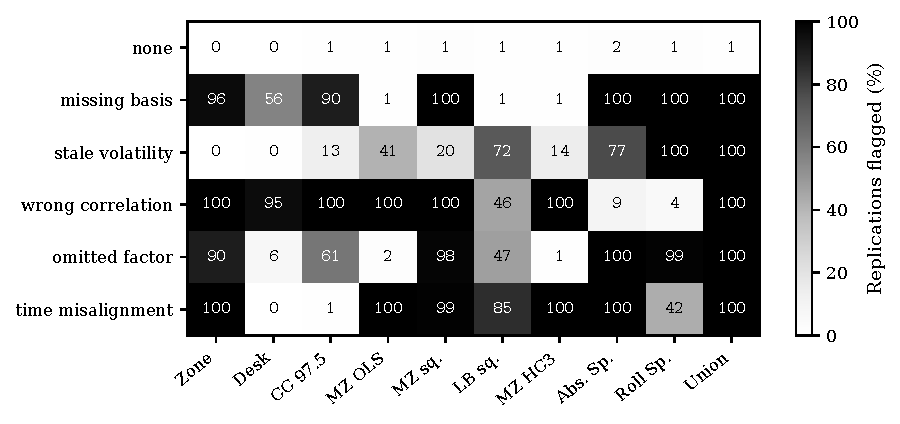
\includegraphics[width=0.92\linewidth]{detection-map}
\caption{Percent of the 1,000 replications of each C13 variant flagged by each detector at its calibrated size, on the committed bake; darker cells are higher rates, and the stale-volatility row is the one the regulatory zone does not flag.}
\label{fig:detection-map}
\end{figure}

\subsection{Stability across independent bakes}
\label{sec:results-repeats}

The committed bake is one draw of 1,000 desk-years per variant.
Table~\ref{tab:repeats} gives the mean and the standard deviation of each rate over five further bakes of 1,000, drawn under other case seeds, with the thresholds unchanged.
The stale-volatility rates are stable: the union flags $99.9\pm0.2$\% and the rolling-mean statistic alone $100.0\pm0.0$\%, the absolute-value statistic $75.3\pm0.7$\%, the Ljung--Box statistic $71.8\pm0.9$\%, the recalibrated Spearman correlation of the levels $56.8\pm0.8$\% and the regulatory zone $0.0\pm0.0$\%.
The false-alarm rate of the union on five fresh null bakes is $1.0\pm0.3$\%, that of the rolling-mean statistic $0.8\pm0.3$\% and that of the absolute-value statistic $1.0\pm0.2$\%, so the 1.6\% of the committed bake for the last is a draw at the upper end of that spread and not a drift.
The weak cells repeat too: the rolling-mean statistic flags the wrong correlation in $4.8\pm0.5$\% and the time misalignment in $42.9\pm0.2$\%.
Across the table the standard deviation over bakes never exceeds 2 percentage points.

\begin{table*}[htbp]
\centering
\scriptsize\setlength{\tabcolsep}{3pt}
\caption{Mean and standard deviation, in percent, of each detector's flag rate over five further independent bakes of 1,000 replications per variant (case seeds 23, 33, 43, 53 and 63), with the thresholds of the calibration null unchanged. The no-deficiency column is the false-alarm rate on five fresh null bakes.}
\label{tab:repeats}
\resizebox{\textwidth}{!}{%
\begin{tabular}{p{4.1cm}cccccc}
\toprule
Detector & No deficiency & Missing basis & Stale volatility (20 days) & Wrong correlation & Omitted factor & Time misalignment \\
\midrule
Regulatory zone, amber or red & $0.0\pm0.0$ & $94.9\pm0.5$ & $0.0\pm0.0$ & $100.0\pm0.0$ & $90.1\pm0.8$ & $100.0\pm0.0$ \\
\relax Spearman of levels, threshold recalibrated at 1\% & $0.9\pm0.3$ & $100.0\pm0.0$ & $56.8\pm0.8$ & $7.8\pm0.8$ & $100.0\pm0.0$ & $100.0\pm0.0$ \\
Desk back-test over its limit & $0.0\pm0.0$ & $58.4\pm1.9$ & $0.6\pm0.2$ & $96.0\pm0.5$ & $6.3\pm1.0$ & $0.0\pm0.0$ \\
\relax Christoffersen conditional coverage, 97.5\% & $0.8\pm0.4$ & $91.2\pm1.3$ & $12.4\pm0.4$ & $100.0\pm0.1$ & $61.5\pm1.6$ & $1.0\pm0.1$ \\
MZ Wald, OLS covariance & $0.8\pm0.4$ & $1.2\pm0.4$ & $38.7\pm1.5$ & $100.0\pm0.0$ & $1.9\pm0.6$ & $100.0\pm0.0$ \\
Ljung--Box on the squared residual & $0.9\pm0.2$ & $0.9\pm0.1$ & $71.8\pm0.9$ & $45.0\pm0.8$ & $50.7\pm1.7$ & $84.4\pm1.1$ \\
MZ Wald, HC3 (proposed) & $0.8\pm0.3$ & $1.1\pm0.3$ & $13.6\pm0.9$ & $100.0\pm0.0$ & $0.9\pm0.4$ & $100.0\pm0.0$ \\
Spearman of absolute values (proposed) & $1.0\pm0.2$ & $100.0\pm0.0$ & $75.3\pm0.7$ & $8.8\pm0.8$ & $100.0\pm0.0$ & $100.0\pm0.0$ \\
Spearman of 20-day rolling means (proposed) & $0.8\pm0.3$ & $99.9\pm0.1$ & $100.0\pm0.0$ & $4.8\pm0.5$ & $98.5\pm0.3$ & $42.9\pm0.2$ \\
\relax Union of the three proposed, family 1\% & $1.0\pm0.3$ & $100.0\pm0.0$ & $99.9\pm0.2$ & $100.0\pm0.0$ & $100.0\pm0.0$ & $100.0\pm0.0$ \\
\bottomrule
\end{tabular}}
\end{table*}


\subsection{The age of the volatility input}
\label{sec:results-lag}

Figure~\ref{fig:mechanism} shows the mechanism on one desk-year of each kind: when the risk model's volatility is twenty days old, the 20-day mean of $|\RTPL|$ follows the 20-day mean of $|\HPL|$ with a delay of the order of the lag.
The correlation of the two rolling means is 0.994 on average on the desks with no deficiency and 0.691 on the stale desks.

\begin{figure}[htbp]
\centering
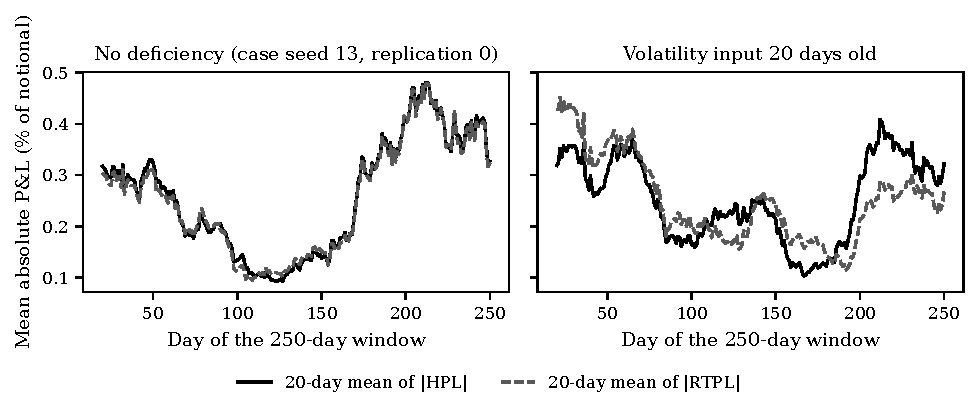
\includegraphics[width=\linewidth]{mechanism}
\caption{Twenty-day rolling means of the absolute hypothetical and risk-theoretical profit and loss of one desk-year with no deficiency (left) and of one desk-year whose risk model uses a volatility twenty days old (right), under the committed generator, in percent of the desk notional.}
\label{fig:mechanism}
\end{figure}

Table~\ref{tab:lag-ladder} and Figure~\ref{fig:power-by-lag} give the rates as the lag grows.
The regulatory zone flags nothing until a lag of 40 days (0.2\%) and flags 5.1\% at 80 days; the desk back-test flags 3.9\% and 13.5\% at the same lags.
The rolling-mean statistic flags 5.7\% at a lag of 2 days, 57.6\% at 5, 97.5\% at 10, 99.9\% at 20 and 100.0\% at 40 and 80 days; the union is a little lower at the short lags (2.9\% and 37.3\% at 2 and 5 days) because the Bonferroni split places each statistic at 0.333\%.
The Ljung--Box statistic rises more slowly (9.0, 26.1, 49.2, 71.9, 82.6 and 86.8\%), the absolute-value statistic is strong from 20 days (76.7\% and above) and weak at 5 and 10 days (4.5 and 25.6\%), and the Wald statistic with the HC3 covariance needs 80 days to flag 45.2\%.
The mean of the Wald statistic goes from 2.05 on the desks with no deficiency to 2.07, 2.54, 3.35, 4.97, 9.04 and 18.78 at the six lags, so the regression component moves in the right direction and slowly, as Proposition~\ref{prop:slope} implies.
The flag rate of the rolling-mean statistic is non-decreasing in the lag over the six lags, so H4 holds on this range.

\begin{table}[htbp]
\centering
\footnotesize
\renewcommand{\arraystretch}{1.1}
\caption{Percent of 1,000 replications flagged, over the 95\% Wilson interval, as the age of the volatility input of the risk model grows from 2 to 80 days (stale-volatility variant, committed seeds; the 20-day row is the committed variant). The first panel holds the regulatory zone and the published comparators, the second the proposed components and their union. Zone is the regulatory zone, Desk the desk back-test limit, CC the Christoffersen conditional coverage, MZ the Mincer--Zarnowitz Wald test with the OLS or HC3 covariance, LB the Ljung--Box test and Sp. the Spearman statistic.}
\label{tab:lag-ladder}
\begin{tabular}{rccccc}
\toprule
Lag (days) & Zone & Desk & CC 97.5 & MZ OLS & LB sq. \\
\midrule
2 & \begin{tabular}[t]{@{}c@{}}0.0\\(0.0--0.4)\end{tabular} & \begin{tabular}[t]{@{}c@{}}0.0\\(0.0--0.4)\end{tabular} & \begin{tabular}[t]{@{}c@{}}1.8\\(1.1--2.8)\end{tabular} & \begin{tabular}[t]{@{}c@{}}5.5\\(4.2--7.1)\end{tabular} & \begin{tabular}[t]{@{}c@{}}9.0\\(7.4--10.9)\end{tabular} \\ \addlinespace[0.8ex]
5 & \begin{tabular}[t]{@{}c@{}}0.0\\(0.0--0.4)\end{tabular} & \begin{tabular}[t]{@{}c@{}}0.0\\(0.0--0.4)\end{tabular} & \begin{tabular}[t]{@{}c@{}}2.8\\(1.9--4.0)\end{tabular} & \begin{tabular}[t]{@{}c@{}}15.1\\(13.0--17.5)\end{tabular} & \begin{tabular}[t]{@{}c@{}}26.1\\(23.5--28.9)\end{tabular} \\ \addlinespace[0.8ex]
10 & \begin{tabular}[t]{@{}c@{}}0.0\\(0.0--0.4)\end{tabular} & \begin{tabular}[t]{@{}c@{}}0.0\\(0.0--0.4)\end{tabular} & \begin{tabular}[t]{@{}c@{}}5.4\\(4.2--7.0)\end{tabular} & \begin{tabular}[t]{@{}c@{}}25.6\\(23.0--28.4)\end{tabular} & \begin{tabular}[t]{@{}c@{}}49.2\\(46.1--52.3)\end{tabular} \\ \addlinespace[0.8ex]
20 & \begin{tabular}[t]{@{}c@{}}0.0\\(0.0--0.4)\end{tabular} & \begin{tabular}[t]{@{}c@{}}0.5\\(0.2--1.2)\end{tabular} & \begin{tabular}[t]{@{}c@{}}12.7\\(10.8--14.9)\end{tabular} & \begin{tabular}[t]{@{}c@{}}41.0\\(38.0--44.1)\end{tabular} & \begin{tabular}[t]{@{}c@{}}71.9\\(69.0--74.6)\end{tabular} \\ \addlinespace[0.8ex]
40 & \begin{tabular}[t]{@{}c@{}}0.2\\(0.1--0.7)\end{tabular} & \begin{tabular}[t]{@{}c@{}}3.9\\(2.9--5.3)\end{tabular} & \begin{tabular}[t]{@{}c@{}}27.1\\(24.4--29.9)\end{tabular} & \begin{tabular}[t]{@{}c@{}}54.6\\(51.5--57.7)\end{tabular} & \begin{tabular}[t]{@{}c@{}}82.6\\(80.1--84.8)\end{tabular} \\ \addlinespace[0.8ex]
80 & \begin{tabular}[t]{@{}c@{}}5.1\\(3.9--6.6)\end{tabular} & \begin{tabular}[t]{@{}c@{}}13.5\\(11.5--15.8)\end{tabular} & \begin{tabular}[t]{@{}c@{}}40.0\\(37.0--43.1)\end{tabular} & \begin{tabular}[t]{@{}c@{}}67.6\\(64.6--70.4)\end{tabular} & \begin{tabular}[t]{@{}c@{}}86.8\\(84.6--88.8)\end{tabular} \\ \addlinespace[0.8ex]
\bottomrule
\end{tabular}

\vspace{1.5ex}

\begin{tabular}{rcccc}
\toprule
Lag (days) & MZ HC3 & Abs. Sp. & Roll Sp. & Union \\
\midrule
2 & \begin{tabular}[t]{@{}c@{}}0.7\\(0.3--1.4)\end{tabular} & \begin{tabular}[t]{@{}c@{}}1.4\\(0.8--2.3)\end{tabular} & \begin{tabular}[t]{@{}c@{}}5.7\\(4.4--7.3)\end{tabular} & \begin{tabular}[t]{@{}c@{}}2.9\\(2.0--4.1)\end{tabular} \\ \addlinespace[0.8ex]
5 & \begin{tabular}[t]{@{}c@{}}2.4\\(1.6--3.5)\end{tabular} & \begin{tabular}[t]{@{}c@{}}4.5\\(3.4--6.0)\end{tabular} & \begin{tabular}[t]{@{}c@{}}57.6\\(54.5--60.6)\end{tabular} & \begin{tabular}[t]{@{}c@{}}37.3\\(34.4--40.3)\end{tabular} \\ \addlinespace[0.8ex]
10 & \begin{tabular}[t]{@{}c@{}}6.0\\(4.7--7.6)\end{tabular} & \begin{tabular}[t]{@{}c@{}}25.6\\(23.0--28.4)\end{tabular} & \begin{tabular}[t]{@{}c@{}}97.5\\(96.3--98.3)\end{tabular} & \begin{tabular}[t]{@{}c@{}}94.0\\(92.4--95.3)\end{tabular} \\ \addlinespace[0.8ex]
20 & \begin{tabular}[t]{@{}c@{}}14.2\\(12.2--16.5)\end{tabular} & \begin{tabular}[t]{@{}c@{}}76.7\\(74.0--79.2)\end{tabular} & \begin{tabular}[t]{@{}c@{}}99.9\\(99.4--100.0)\end{tabular} & \begin{tabular}[t]{@{}c@{}}99.9\\(99.4--100.0)\end{tabular} \\ \addlinespace[0.8ex]
40 & \begin{tabular}[t]{@{}c@{}}28.7\\(26.0--31.6)\end{tabular} & \begin{tabular}[t]{@{}c@{}}94.1\\(92.5--95.4)\end{tabular} & \begin{tabular}[t]{@{}c@{}}100.0\\(99.6--100.0)\end{tabular} & \begin{tabular}[t]{@{}c@{}}100.0\\(99.6--100.0)\end{tabular} \\ \addlinespace[0.8ex]
80 & \begin{tabular}[t]{@{}c@{}}45.2\\(42.1--48.3)\end{tabular} & \begin{tabular}[t]{@{}c@{}}96.2\\(94.8--97.2)\end{tabular} & \begin{tabular}[t]{@{}c@{}}100.0\\(99.6--100.0)\end{tabular} & \begin{tabular}[t]{@{}c@{}}100.0\\(99.6--100.0)\end{tabular} \\ \addlinespace[0.8ex]
\bottomrule
\end{tabular}
\end{table}


\begin{figure}[htbp]
\centering
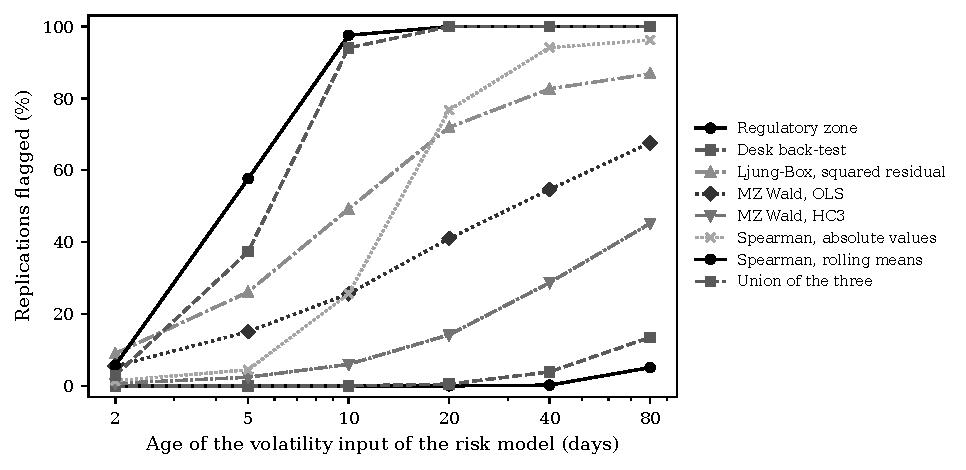
\includegraphics[width=0.86\linewidth]{power-by-lag}
\caption{Percent of 1,000 stale-volatility replications flagged by each detector against the age of the volatility input of the risk model in days (logarithmic axis), committed seeds; the regulatory zone and the desk back-test are near zero over the range where the rolling-mean statistic rises to 100\%.}
\label{fig:power-by-lag}
\end{figure}

\begin{figure}[htbp]
\centering
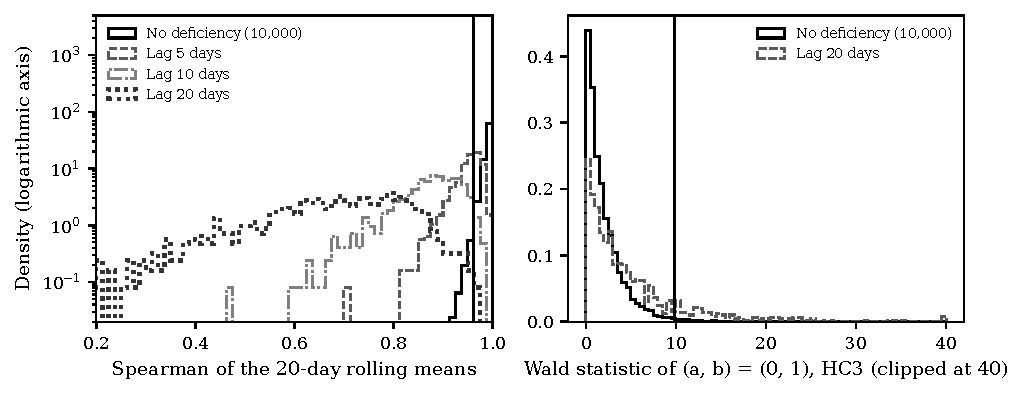
\includegraphics[width=\linewidth]{statistic-distributions}
\caption{Left: distribution of the rolling-mean Spearman statistic on the 10,000 null desk-years and on 1,000 stale-volatility desk-years at lags of 5, 10 and 20 days, with the 1\% critical value as a vertical line. Right: distribution of the HC3 Wald statistic on the null and at a lag of 20 days, clipped at 40, with its critical value.}
\label{fig:distributions}
\end{figure}

Figure~\ref{fig:distributions} shows why the two statistics differ: at a lag of 20 days the distribution of the rolling-mean statistic leaves the null almost entirely, whereas the distribution of the Wald statistic keeps most of its mass inside the null.

\subsection{A threshold-free comparison}
\label{sec:results-auc}

A detector's rate depends on its threshold; the area under the ROC curve does not.
Table~\ref{tab:auc} gives it for the nine statistics between the stale desks and the held-out null.
The rolling-mean statistic has the largest area at every lag: 0.976 at 5 days, 0.999 at 10 and 1.000 at 20 (0.9999 to 1.0000 at 20 days), against 0.837, 0.946 and 0.988 for the absolute-value statistic, 0.807, 0.925 and 0.980 for the Spearman correlation of the levels, and 0.699, 0.856 and 0.938 for the Ljung--Box statistic.
The Kolmogorov--Smirnov distance has 0.596, 0.680 and 0.785, and the Wald statistic with the HC3 covariance 0.549, 0.613 and 0.677.
The Spearman correlation of the levels has a large area, 0.980 at 20 days, while the regulatory zone flags nothing on this desk: the information is in the statistic, and the thresholds of the zone are what discard it.
Figure~\ref{fig:power-against-size} gives the power against the held-out false-alarm rate: at a lag of 10 days the rolling-mean statistic flags 86.2\% at 0.1\% size and 97.5\% at 1\%, while the Spearman correlation of the levels flags 1.3\% and 11.3\% at the same sizes.

\begin{table}[htbp]
\centering
\footnotesize
\caption{Area under the ROC curve of each statistic for separating 1,000 stale-volatility replications at the stated lag from the 1,000 held-out replications with no deficiency, with the 95\% percentile bootstrap interval (1,000 resamples); the area does not depend on any threshold, so it compares the statistics before calibration.}
\label{tab:auc}
\begin{tabular}{lccc}
\toprule
Statistic & Lag 5 days & Lag 10 days & Lag 20 days \\
\midrule
Spearman of 20-day rolling means & 0.976 (0.970--0.981) & 0.999 (0.998--1.000) & 1.000 (1.000--1.000) \\
Spearman of absolute values & 0.837 (0.818--0.855) & 0.946 (0.936--0.956) & 0.988 (0.983--0.991) \\
MZ Wald, HC3 & 0.549 (0.523--0.573) & 0.613 (0.590--0.639) & 0.677 (0.653--0.699) \\
MZ Wald, OLS covariance & 0.683 (0.659--0.706) & 0.749 (0.728--0.770) & 0.800 (0.780--0.819) \\
MZ Wald on squares & 0.580 (0.552--0.604) & 0.667 (0.640--0.690) & 0.786 (0.765--0.805) \\
Ljung--Box on squared residual & 0.699 (0.675--0.722) & 0.856 (0.837--0.872) & 0.938 (0.926--0.948) \\
Christoffersen conditional coverage & 0.541 (0.517--0.565) & 0.609 (0.582--0.634) & 0.692 (0.669--0.715) \\
KS distance (regulatory) & 0.596 (0.574--0.621) & 0.680 (0.658--0.703) & 0.785 (0.767--0.804) \\
Spearman of levels (regulatory) & 0.807 (0.788--0.827) & 0.925 (0.913--0.937) & 0.980 (0.974--0.985) \\
\bottomrule
\end{tabular}
\end{table}


\begin{figure}[htbp]
\centering
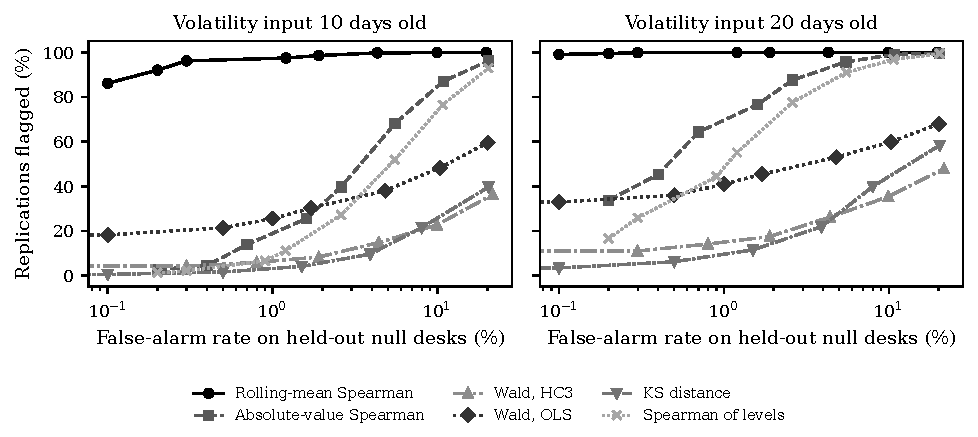
\includegraphics[width=\linewidth]{power-against-size}
\caption{Percent of stale-volatility replications flagged, at lags of 10 days (left) and 20 days (right), against the false-alarm rate on 1,000 held-out null desk-years (logarithmic axis), for sizes of 0.1\% to 20\% read from the 10,000 null desk-years; each curve is one statistic.}
\label{fig:power-against-size}
\end{figure}

\subsection{Defects the rank statistics cannot see}
\label{sec:results-misscale}

Table~\ref{tab:mis-scale} tests H5 on the no-deficiency desk with a constant defect planted in RTPL.
A mis-scale of 10\% in either direction gives a mean fitted slope of 1.111 or 0.909, the values $1/c$ of Proposition~\ref{prop:invariance}, and the Wald test flags 100.0\% of the replications; the regulatory zone flags 0.0\%, and the two rank statistics keep their false-alarm rates of 1.6\% and 1.2\%, unchanged by the rescaling.
A mis-scale of 20 or 25\% is flagged by the zone in 16.2\% and 8.4\%, and by the Wald test in 100.0\%.
A level error is seen by the rank statistics only when large: a shift of 0.1 standard deviations of the HPL is flagged by the Wald test in 100.0\%, by the zone in 18.2\%, by the absolute-value statistic in 26.0\% and by the rolling-mean statistic in 7.9\%, and a shift of 0.2 standard deviations by the zone in 97.3\% and by the rolling-mean statistic in 39.4\%.
H5 holds, and the table shows the role of the regression component: the two regression components, with either covariance, are the only detectors with full power against a constant mis-scale of 10\%.

\begin{table*}[htbp]
\centering
\scriptsize\setlength{\tabcolsep}{3pt}
\caption{Percent of 1,000 replications flagged, with the 95\% Wilson interval, when a constant mis-scale or a constant level error is planted in the risk-theoretical P\&L of the no-deficiency desk (case seed 13), with the mean Mincer--Zarnowitz slope of HPL on RTPL; every detector of the main comparison was run on these desks and the columns are the ones that respond (the desk back-test, the Christoffersen test and the recalibrated Spearman correlation of the levels flag at most 0.0\%, 0.8\% and 1.2\% in every row). The rank statistics are unchanged by a positive rescaling.}
\label{tab:mis-scale}
\resizebox{\textwidth}{!}{%
\begin{tabular}{lrccccccccc}
\toprule
Defect planted in the null desk & Mean slope & Zone & KS recal. & MZ OLS & MZ HC3 & MZ squares & LB sq. & Abs. Sp. & Roll Sp. & Union \\
\midrule
RTPL times 0.80 & 1.250 & 16.2 (14.0--18.6) & 100.0 (99.6--100.0) & 100.0 (99.6--100.0) & 100.0 (99.6--100.0) & 100.0 (99.6--100.0) & 34.3 (31.4--37.3) & 1.6 (1.0--2.6) & 1.2 (0.7--2.1) & 100.0 (99.6--100.0) \\
RTPL times 0.90 & 1.111 & 0.0 (0.0--0.4) & 34.9 (32.0--37.9) & 100.0 (99.6--100.0) & 100.0 (99.6--100.0) & 100.0 (99.6--100.0) & 11.3 (9.5--13.4) & 1.6 (1.0--2.6) & 1.2 (0.7--2.1) & 100.0 (99.6--100.0) \\
RTPL times 1.10 & 0.909 & 0.0 (0.0--0.4) & 12.1 (10.2--14.3) & 100.0 (99.6--100.0) & 100.0 (99.6--100.0) & 100.0 (99.6--100.0) & 11.4 (9.6--13.5) & 1.6 (1.0--2.6) & 1.2 (0.7--2.1) & 100.0 (99.6--100.0) \\
RTPL times 1.25 & 0.800 & 8.4 (6.8--10.3) & 100.0 (99.6--100.0) & 100.0 (99.6--100.0) & 100.0 (99.6--100.0) & 100.0 (99.6--100.0) & 39.6 (36.6--42.7) & 1.6 (1.0--2.6) & 1.2 (0.7--2.1) & 100.0 (99.6--100.0) \\
RTPL shifted by 0.1 sd of HPL & 1.000 & 18.2 (15.9--20.7) & 97.8 (96.7--98.5) & 100.0 (99.6--100.0) & 100.0 (99.6--100.0) & 2.8 (1.9--4.0) & 1.1 (0.6--2.0) & 26.0 (23.4--28.8) & 7.9 (6.4--9.7) & 100.0 (99.6--100.0) \\
RTPL shifted by 0.2 sd of HPL & 1.000 & 97.3 (96.1--98.1) & 100.0 (99.6--100.0) & 100.0 (99.6--100.0) & 100.0 (99.6--100.0) & 13.6 (11.6--15.9) & 0.7 (0.3--1.4) & 95.2 (93.7--96.4) & 39.4 (36.4--42.5) & 100.0 (99.6--100.0) \\
\bottomrule
\end{tabular}}
\end{table*}


\subsection{Size on desks that differ from the calibration null}
\label{sec:results-altnull}

Table~\ref{tab:alt-nulls} tests H3.
With the thresholds of the calibration null unchanged, the false-alarm rate of the union is 0.2\% when the volatility is less persistent (0.90) and 0.7\% when it is less dispersed (0.20), both at or below the stated size, and 0.3\% when the pricing noise is smaller.
It exceeds the stated size when the volatility is more persistent or more dispersed: 4.0\% (3.0 to 5.4\%) at a persistence of 0.995 and 6.2\% (4.9 to 7.9\%) at a dispersion of 0.50, where the absolute-value statistic alone has 8.5\% (6.9 to 10.4\%).
When the pricing noise is 30\% of the factor profit and loss the union flags 99.0\% (98.2 to 99.5\%) of desks with no deficiency, the absolute-value statistic 99.7\% and the rolling-mean statistic 63.5\%, while the Wald statistic with the HC3 covariance stays between 1.1 and 1.7\% and the Ljung--Box statistic at 1.1\% in every row.
H3 fails.
The rank statistics read the agreement of two scales, and a larger pricing noise is a real, if benign, loss of agreement between the pricing and the risk models; the calibration null has to be the desk's own, with its own noise, as Proposition~\ref{prop:size} requires through exchangeability.
Figure~\ref{fig:alt-null} gives the rates on a logarithmic scale.

\begin{table}[htbp]
\centering
\footnotesize
\renewcommand{\arraystretch}{1.1}
\caption{False-alarm rate in percent, over the 95\% Wilson interval, of each detector on 1,000 desk-years of a desk with no deficiency whose generator differs from the calibration null in one parameter, with every threshold taken unchanged from the calibration null; a rate above 1\% means the stated size does not transfer to that desk.}
\label{tab:alt-nulls}
\begin{tabular}{>{\raggedright\arraybackslash}p{4.4cm}cccc}
\toprule
Null desk & Zone & MZ HC3 & Abs. Sp. & Roll Sp. \\
\midrule
No deficiency, case seed 23 (the generator of the calibration null) & \begin{tabular}[t]{@{}c@{}}0.0\\(0.0--0.4)\end{tabular} & \begin{tabular}[t]{@{}c@{}}1.3\\(0.8--2.2)\end{tabular} & \begin{tabular}[t]{@{}c@{}}0.8\\(0.4--1.6)\end{tabular} & \begin{tabular}[t]{@{}c@{}}0.5\\(0.2--1.2)\end{tabular} \\ \addlinespace[0.8ex]
Volatility persistence 0.90 & \begin{tabular}[t]{@{}c@{}}0.0\\(0.0--0.4)\end{tabular} & \begin{tabular}[t]{@{}c@{}}1.7\\(1.1--2.7)\end{tabular} & \begin{tabular}[t]{@{}c@{}}0.0\\(0.0--0.4)\end{tabular} & \begin{tabular}[t]{@{}c@{}}0.0\\(0.0--0.4)\end{tabular} \\ \addlinespace[0.8ex]
Volatility persistence 0.995 & \begin{tabular}[t]{@{}c@{}}0.0\\(0.0--0.4)\end{tabular} & \begin{tabular}[t]{@{}c@{}}1.5\\(0.9--2.5)\end{tabular} & \begin{tabular}[t]{@{}c@{}}4.3\\(3.2--5.7)\end{tabular} & \begin{tabular}[t]{@{}c@{}}4.6\\(3.5--6.1)\end{tabular} \\ \addlinespace[0.8ex]
Volatility dispersion 0.20 & \begin{tabular}[t]{@{}c@{}}0.0\\(0.0--0.4)\end{tabular} & \begin{tabular}[t]{@{}c@{}}1.5\\(0.9--2.5)\end{tabular} & \begin{tabular}[t]{@{}c@{}}0.0\\(0.0--0.4)\end{tabular} & \begin{tabular}[t]{@{}c@{}}1.2\\(0.7--2.1)\end{tabular} \\ \addlinespace[0.8ex]
Volatility dispersion 0.50 & \begin{tabular}[t]{@{}c@{}}0.0\\(0.0--0.4)\end{tabular} & \begin{tabular}[t]{@{}c@{}}1.1\\(0.6--2.0)\end{tabular} & \begin{tabular}[t]{@{}c@{}}8.5\\(6.9--10.4)\end{tabular} & \begin{tabular}[t]{@{}c@{}}1.3\\(0.8--2.2)\end{tabular} \\ \addlinespace[0.8ex]
Pricing noise 5\% of factor P\&L & \begin{tabular}[t]{@{}c@{}}0.0\\(0.0--0.4)\end{tabular} & \begin{tabular}[t]{@{}c@{}}1.3\\(0.8--2.2)\end{tabular} & \begin{tabular}[t]{@{}c@{}}0.0\\(0.0--0.4)\end{tabular} & \begin{tabular}[t]{@{}c@{}}0.0\\(0.0--0.4)\end{tabular} \\ \addlinespace[0.8ex]
Pricing noise 30\% of factor P\&L & \begin{tabular}[t]{@{}c@{}}1.0\\(0.5--1.8)\end{tabular} & \begin{tabular}[t]{@{}c@{}}1.3\\(0.8--2.2)\end{tabular} & \begin{tabular}[t]{@{}c@{}}99.7\\(99.1--99.9)\end{tabular} & \begin{tabular}[t]{@{}c@{}}63.5\\(60.5--66.4)\end{tabular} \\ \addlinespace[0.8ex]
\bottomrule
\end{tabular}

\vspace{1.5ex}

\begin{tabular}{>{\raggedright\arraybackslash}p{4.4cm}ccc}
\toprule
Null desk & Union & LB sq. & MZ squares \\
\midrule
No deficiency, case seed 23 (the generator of the calibration null) & \begin{tabular}[t]{@{}c@{}}0.8\\(0.4--1.6)\end{tabular} & \begin{tabular}[t]{@{}c@{}}1.1\\(0.6--2.0)\end{tabular} & \begin{tabular}[t]{@{}c@{}}0.7\\(0.3--1.4)\end{tabular} \\ \addlinespace[0.8ex]
Volatility persistence 0.90 & \begin{tabular}[t]{@{}c@{}}0.2\\(0.1--0.7)\end{tabular} & \begin{tabular}[t]{@{}c@{}}1.1\\(0.6--2.0)\end{tabular} & \begin{tabular}[t]{@{}c@{}}1.5\\(0.9--2.5)\end{tabular} \\ \addlinespace[0.8ex]
Volatility persistence 0.995 & \begin{tabular}[t]{@{}c@{}}4.0\\(3.0--5.4)\end{tabular} & \begin{tabular}[t]{@{}c@{}}1.1\\(0.6--2.0)\end{tabular} & \begin{tabular}[t]{@{}c@{}}1.3\\(0.8--2.2)\end{tabular} \\ \addlinespace[0.8ex]
Volatility dispersion 0.20 & \begin{tabular}[t]{@{}c@{}}0.7\\(0.3--1.4)\end{tabular} & \begin{tabular}[t]{@{}c@{}}1.1\\(0.6--2.0)\end{tabular} & \begin{tabular}[t]{@{}c@{}}0.7\\(0.3--1.4)\end{tabular} \\ \addlinespace[0.8ex]
Volatility dispersion 0.50 & \begin{tabular}[t]{@{}c@{}}6.2\\(4.9--7.9)\end{tabular} & \begin{tabular}[t]{@{}c@{}}1.1\\(0.6--2.0)\end{tabular} & \begin{tabular}[t]{@{}c@{}}1.8\\(1.1--2.8)\end{tabular} \\ \addlinespace[0.8ex]
Pricing noise 5\% of factor P\&L & \begin{tabular}[t]{@{}c@{}}0.3\\(0.1--0.9)\end{tabular} & \begin{tabular}[t]{@{}c@{}}1.1\\(0.6--2.0)\end{tabular} & \begin{tabular}[t]{@{}c@{}}0.3\\(0.1--0.9)\end{tabular} \\ \addlinespace[0.8ex]
Pricing noise 30\% of factor P\&L & \begin{tabular}[t]{@{}c@{}}99.0\\(98.2--99.5)\end{tabular} & \begin{tabular}[t]{@{}c@{}}1.1\\(0.6--2.0)\end{tabular} & \begin{tabular}[t]{@{}c@{}}30.2\\(27.4--33.1)\end{tabular} \\ \addlinespace[0.8ex]
\bottomrule
\end{tabular}
\end{table}


\begin{figure}[htbp]
\centering
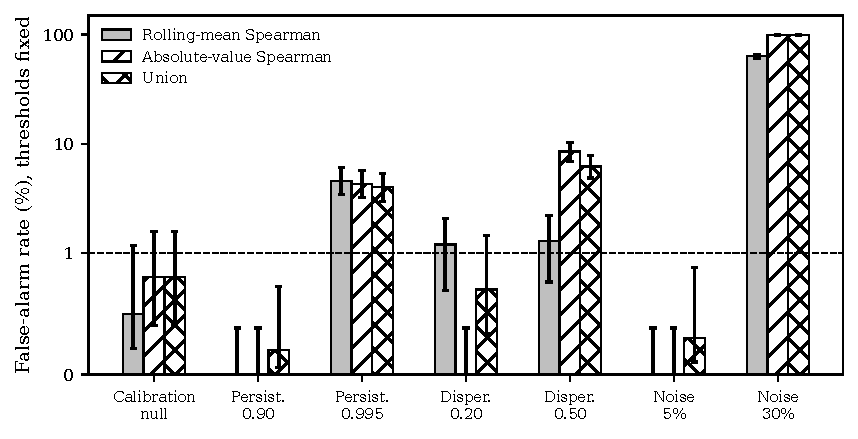
\includegraphics[width=0.88\linewidth]{alternative-nulls}
\caption{False-alarm rate in percent, on a symmetric logarithmic axis, of the rolling-mean statistic, the absolute-value statistic and the union on 1,000 desk-years with nothing planted whose generator differs from the calibration null in one parameter, with the 95\% Wilson interval and the 1\% stated size as a dashed line.}
\label{fig:alt-null}
\end{figure}

\subsection{The predictions}
\label{sec:results-hypotheses}

Table~\ref{tab:hypotheses} gives the outcome of each prediction.
H1 holds by a wide margin: the union flags the stale desk in 99.9\% of replications at a held-out false-alarm rate of 0.9\%, against the criterion of 30\% at a size of at most 1\% and a refutation bound of 10\%; the lower end of its interval, 99.4\%, is far above the criterion, and the size is not above 1\% beyond its sampling interval (0.5 to 1.7\%).
H2 holds in part.
The Wald statistic flags the wrong-correlation variant in 100.0\% of replications, as often as the Kolmogorov--Smirnov distance alone, and the desk with no deficiency at 0.8\%; it does not flag the missing-basis variant (0.9\% against 86.7\% for the distance), for the reason of Corollary~\ref{cor:noise}.
H3 fails, H4 holds and H5 holds, as shown above.

\begin{table*}[htbp]
\centering
\scriptsize
\caption{The five predictions of the experimental design, the criterion each was held to, the measured values on the committed bake or on the experiments of Section~\ref{sec:experimental-design}, and whether each held; H1 is the acceptance and refutation criterion fixed for the method before this evaluation and H2 the second clause of the research brief that proposed it.}
\label{tab:hypotheses}
\begin{tabular}{lp{4.8cm}p{6.2cm}l}
\toprule
Id & Prediction & Measured & Outcome \\
\midrule
H1 & \relax At a size of at most 1\%, the stale-volatility model is flagged in at least 30\% of replications; refuted below 10\% & \relax union 99.9 (99.4--100.0)\% at held-out size 0.9 (0.5--1.7)\%; regulatory zone 0.0\% & held \\
H2 & The Wald test flags wrong-correlation and missing-basis at least as often as the KS distance alone, and the no-deficiency desk at most at the stated rate & \relax wrong correlation 100.0\% against 100.0\%; missing basis 0.9\% against 86.7\%; no deficiency 0.8\% & held in part \\
H3 & \relax The false-alarm rate of the union stays at most 1\% on desks that differ from the calibration null & \relax 4.0\% (persistence 0.995), 6.2\% (dispersion 0.50), 99.0\% (pricing noise 30\%) & failed \\
H4 & The flag rate of the rolling-mean statistic rises with the age of the volatility input & \relax rates 5.7, 57.6, 97.5, 99.9, 100.0, 100.0\% at 2, 5, 10, 20, 40 and 80 days & held \\
H5 & The complement flags a constant mis-scale that the regulatory zone does not & \relax Wald 100.0\% against zone 0.0\% at a 10\% mis-scale & held \\
\bottomrule
\end{tabular}
\end{table*}


\subsection{Checks of the propositions}
\label{sec:results-theory}

Table~\ref{tab:theory-size} compares Proposition~\ref{prop:size} with the false-alarm rate of the critical value read from $N$ Gaussian null draws, repeated 2,000 to 20,000 times: the mean and the standard deviation agree with the proposition to the third significant figure (for $N=10{,}000$ and $p=1\%$, 1.012\% against 1.010\% and 0.100 against 0.100 points).
Table~\ref{tab:theory-loo} makes the check on the real null: each of the ten blocks of 1,000 null desk-years is flagged with the critical value calibrated on the other 9,000, and the mean over the ten folds is 1.01, 0.99 and 1.00\% for the Wald, absolute-value and rolling-mean statistics against 1.011\% predicted, with a standard deviation over folds of 0.31 to 0.35 points, close to the 0.31 points that a rate of 1\% on 1,000 desk-years carries.

\begin{table*}[htbp]
\centering
\footnotesize
\caption{Out-of-sample false-alarm rate, in percent, of the critical value that is the (k+1)-th most extreme of N independent standard normal null values: the mean and standard deviation that Proposition 1 gives and the values measured over the stated number of independent calibration draws.}
\label{tab:theory-size}
\begin{tabular}{rrrrrrrr}
\toprule
N & p (\%) & k & Draws & Mean, Prop. 1 & Mean, simulated & SD, Prop. 1 & SD, simulated \\
\midrule
100 & 5 & 5 & 20,000 & 5.941 & 5.931 & 2.341 & 2.352 \\
1,000 & 1 & 10 & 20,000 & 1.099 & 1.101 & 0.329 & 0.328 \\
1,000 & 5 & 50 & 20,000 & 5.095 & 5.090 & 0.695 & 0.695 \\
10,000 & 1 & 100 & 2,000 & 1.010 & 1.012 & 0.100 & 0.100 \\
10,000 & 0.333 & 33 & 2,000 & 0.340 & 0.338 & 0.058 & 0.058 \\
\bottomrule
\end{tabular}
\end{table*}


\begin{table}[htbp]
\centering
\footnotesize
\caption{Leave-one-block-out check of Proposition 1 on the real null: each of the ten blocks of 1,000 null desk-years is flagged with the critical value calibrated on the other 9,000; the table gives, in percent, the value Proposition 1 predicts for a calibration of 9,000 and the mean and standard deviation of the ten measured rates.}
\label{tab:theory-loo}
\begin{tabular}{>{\raggedright\arraybackslash}p{6.4cm}rrr}
\toprule
Statistic and size & Mean, Prop. 1 & Mean over 10 folds & SD over 10 folds \\
\midrule
\relax Wald, HC3 (1\% per statistic) & 1.011 & 1.010 & 0.354 \\
\relax Wald, HC3 (0.333\% per statistic) & 0.344 & 0.340 & 0.165 \\
\relax absolute-value Spearman (1\% per statistic) & 1.011 & 0.990 & 0.314 \\
\relax absolute-value Spearman (0.333\% per statistic) & 0.344 & 0.350 & 0.196 \\
\relax rolling-mean Spearman (1\% per statistic) & 1.011 & 1.000 & 0.320 \\
\relax rolling-mean Spearman (0.333\% per statistic) & 0.344 & 0.330 & 0.263 \\
\bottomrule
\end{tabular}
\end{table}


Table~\ref{tab:theory-slope-corr} and Figure~\ref{fig:theory-check} compare Propositions~\ref{prop:slope} and~\ref{prop:rolling} with simulation.
On windows of 100,000 days the simulated slope equals Equation~\eqref{eq:slope} to within 1.2 standard errors at every lag (0.9603 against 0.9601 at 20 days) and the simulated correlation of the rolling means equals Equation~\eqref{eq:rolling-corr} to within 0.006 (0.8084 $\pm$ 0.0014 against 0.8054 at 20 days; 0.6021 $\pm$ 0.0025 against 0.5969 at 40).
On the 250-day windows of the desk the mean correlation is lower, 0.6946 $\pm$ 0.0023 at 20 days in the noise-free model and 0.6908 on the committed desks with their pricing noise, and the mean slope is above the closed form by 0.003 at 20 days (0.9633 against 0.9601) and by 0.016 at 80 days, which is the small-sample bias of a ratio of sample moments of a persistent process.
The closed forms are population quantities, the 250-day desk is a sample of them, and the thresholds are calibrated on the sample law, so the decision never depends on the population value.

\begin{table}[htbp]
\centering
\footnotesize
\renewcommand{\arraystretch}{1.1}
\caption{The Mincer--Zarnowitz slope and the Pearson correlation of the 20-day rolling means of the absolute series at each lag of the volatility input: the closed forms of Propositions 2 and 3, the mean over 1,000 C13 desk-years of 250 days (with its standard error, and for the slope its standard deviation over desk-years), and an independent simulation of the noise-free model on windows of 100,000 and of 250 days (mean and standard error over 20 and 4,000 windows). The first panel is the slope, the second the correlation.}
\label{tab:theory-slope-corr}
\begin{tabular}{rcccc}
\toprule
Lag & \shortstack{Closed\\form} & \shortstack{100,000-day\\windows} & \shortstack{C13\\mean} & \shortstack{C13\\sd} \\
\midrule
0 & 1.0000 & $1.0000\pm0.0000$ & $1.0002\pm0.0002$ & 0.0069 \\ \addlinespace[0.8ex]
2 & 0.9952 & $0.9951\pm0.0001$ & $0.9955\pm0.0004$ & 0.0128 \\ \addlinespace[0.8ex]
5 & 0.9883 & $0.9885\pm0.0002$ & $0.9882\pm0.0006$ & 0.0202 \\ \addlinespace[0.8ex]
10 & 0.9778 & $0.9776\pm0.0002$ & $0.9788\pm0.0010$ & 0.0310 \\ \addlinespace[0.8ex]
20 & 0.9601 & $0.9603\pm0.0003$ & $0.9633\pm0.0016$ & 0.0508 \\ \addlinespace[0.8ex]
40 & 0.9344 & $0.9346\pm0.0005$ & $0.9426\pm0.0026$ & 0.0836 \\ \addlinespace[0.8ex]
80 & 0.9065 & $0.9063\pm0.0009$ & $0.9228\pm0.0042$ & 0.1312 \\ \addlinespace[0.8ex]
\bottomrule
\end{tabular}

\vspace{1.5ex}

\begin{tabular}{rcccc}
\toprule
Lag & \shortstack{Closed\\form} & \shortstack{100,000-day\\windows} & \shortstack{250-day\\windows} & \shortstack{C13\\mean} \\
\midrule
0 & 1.0000 & $1.0000\pm0.0000$ & $1.0000\pm0.0000$ & $0.9942\pm0.0002$ \\ \addlinespace[0.8ex]
2 & 0.9959 & $0.9960\pm0.0000$ & $0.9932\pm0.0001$ & $0.9874\pm0.0003$ \\ \addlinespace[0.8ex]
5 & 0.9800 & $0.9802\pm0.0001$ & $0.9666\pm0.0003$ & $0.9610\pm0.0007$ \\ \addlinespace[0.8ex]
10 & 0.9333 & $0.9340\pm0.0005$ & $0.8909\pm0.0009$ & $0.8866\pm0.0018$ \\ \addlinespace[0.8ex]
20 & 0.8054 & $0.8084\pm0.0014$ & $0.6946\pm0.0023$ & $0.6908\pm0.0044$ \\ \addlinespace[0.8ex]
40 & 0.5969 & $0.6021\pm0.0025$ & $0.4284\pm0.0038$ & $0.4203\pm0.0076$ \\ \addlinespace[0.8ex]
80 & 0.3717 & $0.3732\pm0.0039$ & $0.2286\pm0.0050$ & $0.2089\pm0.0099$ \\ \addlinespace[0.8ex]
\bottomrule
\end{tabular}
\end{table}


\begin{figure}[htbp]
\centering
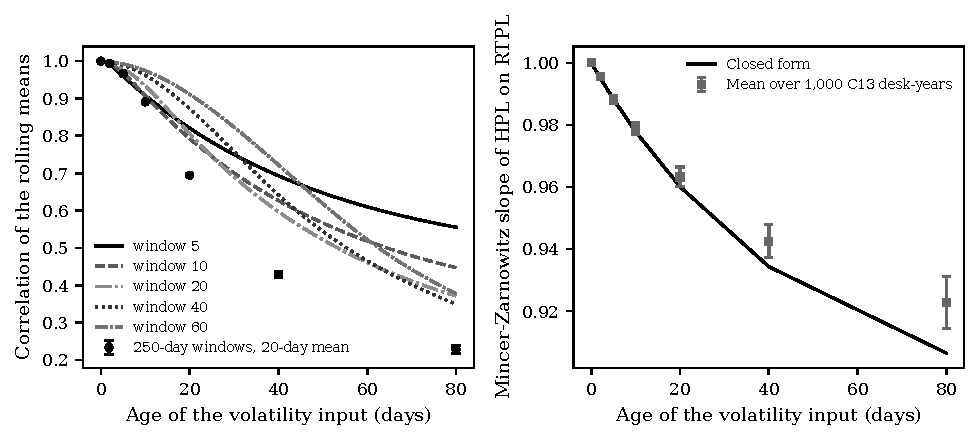
\includegraphics[width=\linewidth]{theory-check}
\caption{Left: the closed-form correlation of the rolling means against the age of the volatility input, for five windows, with the mean and twice the standard error of the simulated 250-day windows for the 20-day mean. Right: the closed-form regression slope of Proposition~\ref{prop:slope} against the mean fitted slope over 1,000 C13 desk-years with twice its standard error.}
\label{fig:theory-check}
\end{figure}

\section{Ablation}
\label{sec:ablation}

Table~\ref{tab:ablation} gives, for each configuration, the held-out false-alarm rate and the detection rate on the stale desk at four lags and on the four other variants, with every configuration calibrated on the same 10,000 null desk-years at a family size of 1\%.
Each row changes one thing from the full complement.

\begin{table}[htbp]
\centering
\footnotesize
\renewcommand{\arraystretch}{1.1}
\caption{Ablation of the complement, first part: held-out false-alarm rate (Size) and detection of the stale-volatility variant at lags of 5, 10, 20 and 40 days (L5 to L40), for the full complement and for each component removed, replaced or changed; every configuration is calibrated on the same 10,000 null desk-years at a family size of 1\% (the no-correction row at 1\% per statistic); percent of 1,000 replications flagged, over the 95\% Wilson interval.}
\label{tab:ablation}
\begin{tabular}{>{\raggedright\arraybackslash}p{3.5cm}ccccc}
\toprule
Configuration & Size & L5 & L10 & L20 & L40 \\
\midrule
Full complement (three statistics, Bonferroni) & \begin{tabular}[t]{@{}c@{}}0.9\\(0.5--1.7)\end{tabular} & \begin{tabular}[t]{@{}c@{}}37.3\\(34.4--40.3)\end{tabular} & \begin{tabular}[t]{@{}c@{}}94.0\\(92.4--95.3)\end{tabular} & \begin{tabular}[t]{@{}c@{}}99.9\\(99.4--100.0)\end{tabular} & \begin{tabular}[t]{@{}c@{}}100.0\\(99.6--100.0)\end{tabular} \\ \addlinespace[0.8ex]
Without the Wald test & \begin{tabular}[t]{@{}c@{}}1.0\\(0.5--1.8)\end{tabular} & \begin{tabular}[t]{@{}c@{}}44.5\\(41.4--47.6)\end{tabular} & \begin{tabular}[t]{@{}c@{}}96.3\\(94.9--97.3)\end{tabular} & \begin{tabular}[t]{@{}c@{}}100.0\\(99.6--100.0)\end{tabular} & \begin{tabular}[t]{@{}c@{}}100.0\\(99.6--100.0)\end{tabular} \\ \addlinespace[0.8ex]
Without the absolute-value Spearman & \begin{tabular}[t]{@{}c@{}}0.6\\(0.3--1.3)\end{tabular} & \begin{tabular}[t]{@{}c@{}}44.4\\(41.3--47.5)\end{tabular} & \begin{tabular}[t]{@{}c@{}}96.3\\(94.9--97.3)\end{tabular} & \begin{tabular}[t]{@{}c@{}}99.9\\(99.4--100.0)\end{tabular} & \begin{tabular}[t]{@{}c@{}}100.0\\(99.6--100.0)\end{tabular} \\ \addlinespace[0.8ex]
Without the rolling-mean Spearman & \begin{tabular}[t]{@{}c@{}}1.0\\(0.5--1.8)\end{tabular} & \begin{tabular}[t]{@{}c@{}}3.8\\(2.8--5.2)\end{tabular} & \begin{tabular}[t]{@{}c@{}}17.3\\(15.1--19.8)\end{tabular} & \begin{tabular}[t]{@{}c@{}}67.7\\(64.7--70.5)\end{tabular} & \begin{tabular}[t]{@{}c@{}}92.4\\(90.6--93.9)\end{tabular} \\ \addlinespace[0.8ex]
Wald test alone & \begin{tabular}[t]{@{}c@{}}0.8\\(0.4--1.6)\end{tabular} & \begin{tabular}[t]{@{}c@{}}2.4\\(1.6--3.5)\end{tabular} & \begin{tabular}[t]{@{}c@{}}6.0\\(4.7--7.6)\end{tabular} & \begin{tabular}[t]{@{}c@{}}14.2\\(12.2--16.5)\end{tabular} & \begin{tabular}[t]{@{}c@{}}28.7\\(26.0--31.6)\end{tabular} \\ \addlinespace[0.8ex]
Absolute-value Spearman alone & \begin{tabular}[t]{@{}c@{}}1.6\\(1.0--2.6)\end{tabular} & \begin{tabular}[t]{@{}c@{}}4.5\\(3.4--6.0)\end{tabular} & \begin{tabular}[t]{@{}c@{}}25.6\\(23.0--28.4)\end{tabular} & \begin{tabular}[t]{@{}c@{}}76.7\\(74.0--79.2)\end{tabular} & \begin{tabular}[t]{@{}c@{}}94.1\\(92.5--95.4)\end{tabular} \\ \addlinespace[0.8ex]
Rolling-mean Spearman alone (20 days) & \begin{tabular}[t]{@{}c@{}}1.2\\(0.7--2.1)\end{tabular} & \begin{tabular}[t]{@{}c@{}}57.6\\(54.5--60.6)\end{tabular} & \begin{tabular}[t]{@{}c@{}}97.5\\(96.3--98.3)\end{tabular} & \begin{tabular}[t]{@{}c@{}}99.9\\(99.4--100.0)\end{tabular} & \begin{tabular}[t]{@{}c@{}}100.0\\(99.6--100.0)\end{tabular} \\ \addlinespace[0.8ex]
Rolling-mean Spearman, 5 days & \begin{tabular}[t]{@{}c@{}}1.2\\(0.7--2.1)\end{tabular} & \begin{tabular}[t]{@{}c@{}}91.1\\(89.2--92.7)\end{tabular} & \begin{tabular}[t]{@{}c@{}}99.8\\(99.3--99.9)\end{tabular} & \begin{tabular}[t]{@{}c@{}}100.0\\(99.6--100.0)\end{tabular} & \begin{tabular}[t]{@{}c@{}}100.0\\(99.6--100.0)\end{tabular} \\ \addlinespace[0.8ex]
Rolling-mean Spearman, 10 days & \begin{tabular}[t]{@{}c@{}}1.0\\(0.5--1.8)\end{tabular} & \begin{tabular}[t]{@{}c@{}}82.9\\(80.4--85.1)\end{tabular} & \begin{tabular}[t]{@{}c@{}}99.8\\(99.3--99.9)\end{tabular} & \begin{tabular}[t]{@{}c@{}}100.0\\(99.6--100.0)\end{tabular} & \begin{tabular}[t]{@{}c@{}}100.0\\(99.6--100.0)\end{tabular} \\ \addlinespace[0.8ex]
Rolling-mean Spearman, 40 days & \begin{tabular}[t]{@{}c@{}}1.0\\(0.5--1.8)\end{tabular} & \begin{tabular}[t]{@{}c@{}}24.2\\(21.6--27.0)\end{tabular} & \begin{tabular}[t]{@{}c@{}}83.4\\(81.0--85.6)\end{tabular} & \begin{tabular}[t]{@{}c@{}}98.4\\(97.4--99.0)\end{tabular} & \begin{tabular}[t]{@{}c@{}}99.9\\(99.4--100.0)\end{tabular} \\ \addlinespace[0.8ex]
Rolling-mean Spearman, 60 days & \begin{tabular}[t]{@{}c@{}}1.0\\(0.5--1.8)\end{tabular} & \begin{tabular}[t]{@{}c@{}}15.4\\(13.3--17.8)\end{tabular} & \begin{tabular}[t]{@{}c@{}}61.9\\(58.8--64.9)\end{tabular} & \begin{tabular}[t]{@{}c@{}}94.2\\(92.6--95.5)\end{tabular} & \begin{tabular}[t]{@{}c@{}}98.8\\(97.9--99.3)\end{tabular} \\ \addlinespace[0.8ex]
OLS covariance in place of HC3 & \begin{tabular}[t]{@{}c@{}}1.1\\(0.6--2.0)\end{tabular} & \begin{tabular}[t]{@{}c@{}}44.2\\(41.1--47.3)\end{tabular} & \begin{tabular}[t]{@{}c@{}}95.4\\(93.9--96.5)\end{tabular} & \begin{tabular}[t]{@{}c@{}}100.0\\(99.6--100.0)\end{tabular} & \begin{tabular}[t]{@{}c@{}}100.0\\(99.6--100.0)\end{tabular} \\ \addlinespace[0.8ex]
No multiplicity correction (1\% each) & \begin{tabular}[t]{@{}c@{}}3.3\\(2.4--4.6)\end{tabular} & \begin{tabular}[t]{@{}c@{}}59.4\\(56.3--62.4)\end{tabular} & \begin{tabular}[t]{@{}c@{}}97.9\\(96.8--98.6)\end{tabular} & \begin{tabular}[t]{@{}c@{}}100.0\\(99.6--100.0)\end{tabular} & \begin{tabular}[t]{@{}c@{}}100.0\\(99.6--100.0)\end{tabular} \\ \addlinespace[0.8ex]
Rolling means at 5, 10, 20 and 40 days (Bonferroni) & \begin{tabular}[t]{@{}c@{}}0.5\\(0.2--1.2)\end{tabular} & \begin{tabular}[t]{@{}c@{}}76.7\\(74.0--79.2)\end{tabular} & \begin{tabular}[t]{@{}c@{}}99.5\\(98.8--99.8)\end{tabular} & \begin{tabular}[t]{@{}c@{}}100.0\\(99.6--100.0)\end{tabular} & \begin{tabular}[t]{@{}c@{}}100.0\\(99.6--100.0)\end{tabular} \\ \addlinespace[0.8ex]
Full complement and regulatory zone & \begin{tabular}[t]{@{}c@{}}0.9\\(0.5--1.7)\end{tabular} & \begin{tabular}[t]{@{}c@{}}37.3\\(34.4--40.3)\end{tabular} & \begin{tabular}[t]{@{}c@{}}94.0\\(92.4--95.3)\end{tabular} & \begin{tabular}[t]{@{}c@{}}99.9\\(99.4--100.0)\end{tabular} & \begin{tabular}[t]{@{}c@{}}100.0\\(99.6--100.0)\end{tabular} \\ \addlinespace[0.8ex]
\bottomrule
\end{tabular}
\end{table}


\subsection{What each component contributes}
\label{sec:ablation-components}

Removing the rolling-mean statistic costs the stale-volatility detection: from 37.3, 94.0, 99.9 and 100.0\% at lags of 5, 10, 20 and 40 days to 3.8, 17.3, 67.7 and 92.4\%.
It is the component that carries the result, and it carries it alone: the rolling-mean statistic on its own flags 57.6, 97.5, 99.9 and 100.0\% at its own 1\% size.
Removing the absolute-value statistic costs little on the six variants (the stale detection is unchanged within 0.1 points at 20 days, and the omitted-factor detection falls from 100.0 to 97.3\%), because the rolling-mean statistic and the Wald statistic cover most of what it sees; its single-statistic row shows what it sees alone: 76.7\% at a lag of 20 days, 100.0\% of the missing-basis variant, which the Wald statistic cannot see, and 100.0\% of the omitted-factor variant.
Removing the Wald statistic drops the wrong-correlation detection from 100.0 to 7.4\%, and the only other change is the gain at short lags that the smaller multiplicity split brings (44.5 against 37.3\% at 5 days and 96.3 against 94.0\% at 10); the Wald statistic alone flags the wrong correlation and the time misalignment (100.0\% each) and is blind to the missing basis (0.9\%) and the omitted factor (0.6\%), as the theory predicts.
The regulatory zone flags the wrong correlation and the time misalignment in 100.0\% of replications, so on these six variants the Wald statistic adds nothing that the zone does not already provide; its unique contribution is the constant mis-scale of Table~\ref{tab:mis-scale}, which neither the zone nor the rank statistics see.
Adding the regulatory zone to the union changes no rate in the table, since the zone flags none of the stale desks.
The multiplicity split has a price: with three statistics each at 0.333\% the detection at a lag of 5 days is 37.3\%, and with two statistics (the rows without the Wald or the absolute-value statistic) it is 44.5 and 44.4\%.

\subsection{The window}
\label{sec:ablation-window}

The rolling window was fixed at 20 days before the evaluation, and Table~\ref{tab:ablation} and Figure~\ref{fig:window-ablation} show how the rate depends on it.
At equal size (between 1.0 and 1.2\% held out for every window) shorter windows detect more of the short lags: at a lag of 5 days the rate is 91.1\% for a window of 5 days, 82.9\% for 10, 57.6\% for 20, 24.2\% for 40 and 15.4\% for 60; at a lag of 10 days it is 99.8, 99.8, 97.5, 83.4 and 61.9\%.
Shorter windows also hold the time-misalignment detection (100.0\% at 5 days and 94.5\% at 10, against 42.3\% at 20 and 5.3\% at 60), because a one-day shift of the series is visible in a rolling mean only when the mean is short.
No window helps against the wrong correlation (2.6 to 8.9\%), which is a defect of the cross-sectional aggregation and not of the scale.
Combining four windows (5, 10, 20 and 40 days) by a Bonferroni split over four statistics gives 76.7\% at a lag of 5 days and 99.5\% at 10, at a held-out size of 0.5\% (0.2 to 1.2\%), between the best single window and the default.
The window of 20 days is therefore not the best of the windows tested on these desks.
It is kept as the method's default because it was fixed in advance and because this table was computed on the same committed seeds as the main results: choosing the best window from it would select on the evaluation data, and a change of the default needs an evaluation on desks that this table has not seen.

\begin{figure}[htbp]
\centering
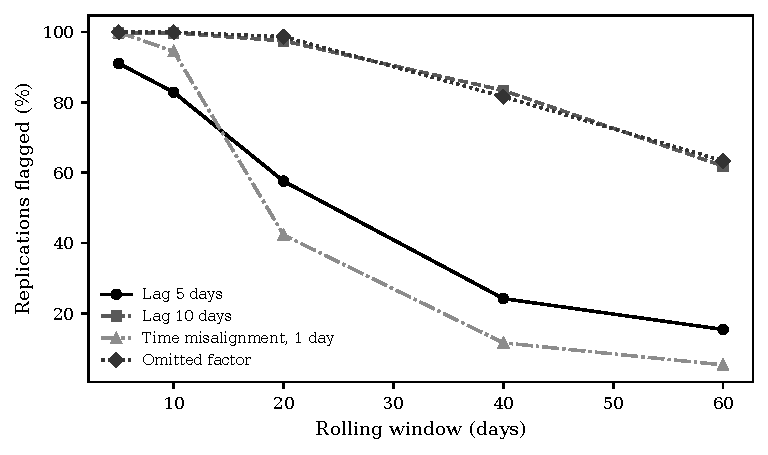
\includegraphics[width=0.86\linewidth]{window-ablation}
\caption{Percent of 1,000 replications flagged by the rolling-mean Spearman statistic against the length of its window in days, at a size of 1\% read from the 10,000 null desk-years, on the stale-volatility desk at lags of 5 and 10 days and on the time-misalignment and omitted-factor variants.}
\label{fig:window-ablation}
\end{figure}

\subsection{The covariance and the multiplicity correction}
\label{sec:ablation-covariance}

The HC3 covariance is motivated by the time-varying volatility of the profit and loss (Section~\ref{sec:method-regression}), and the ablation tests whether it earns its place in the decision.
Replacing it by the ordinary least-squares covariance in the three-statistic union gives a held-out size of 1.1\% against 0.9\% and detection rates of 44.2, 95.4, 100.0 and 100.0\% at lags of 5, 10, 20 and 40 days, against 37.3, 94.0, 99.9 and 100.0\%; the Wald statistic alone flags the stale desk in 41.0\% of replications with the ordinary covariance and in 14.2\% with HC3.
The decision never uses the asymptotic $\chi^2_2$ reference, because its threshold is read from the simulated null, which absorbs the heteroskedasticity either way; the HC3 covariance then gives no gain in power on these desks and costs some, and the choice is kept only because it makes the reference p-value that the engine reports meaningful on a desk whose volatility is not constant.
This is a negative result for the HC3 component of the specification as it stands: a decision read only from the simulated null does not need it.
Removing the multiplicity correction, so that each statistic is calibrated at 1\%, raises the detection at a lag of 5 days from 37.3 to 59.4\% and the held-out size from 0.9\% to 3.3\% (2.4 to 4.6\%), which is the size that three statistics at 1\% each allow; the Bonferroni split keeps the stated family size at the price of about 22 points of power at the shortest lag and none at a lag of 20 days.

\section{Discussion}
\label{sec:discussion}

\subsection{Why the rolling-mean statistic works and the regression does not}
\label{sec:discussion-why}

The stale-volatility deficiency moves the scale of the risk-theoretical profit and loss late and leaves everything else of the desk intact: the sign of each day's move, the order of the moves, the marginal distribution over a year and the conditional mean of HPL given RTPL up to a four per cent tilt.
Each statistic of the regulatory test and the Wald statistic reads one of these preserved features, which is why none of them moves.
The rolling-mean statistic reads the one feature the deficiency changes.
Averaging $|\HPL|$ and $|\RTPL|$ over 20 days removes most of the daily shock that the two series share and leaves the two scale paths, and the correlation of the two paths falls from 0.994 to 0.691 on the desk-years of the generator (Proposition~\ref{prop:rolling} gives 1.000 and 0.805 as population values for the noise-free desk).
The separation between the null and the stale distributions of the statistic is almost complete at a lag of 20 days (area under the curve 1.000), so the threshold matters little there; it matters at short lags, where the two distributions overlap and the calibrated size decides the rate (57.6\% at 5 days).
The regression sees the same deficiency as a slope of 0.960 against 1, which is under one sampling standard deviation of the fitted slope, and so it flags the desk in 14.2\% of replications.

\subsection{Threshold or statistic}
\label{sec:discussion-threshold}

The regulatory zone flags none of the stale desks, and the Spearman correlation of the levels, read at a threshold calibrated to a 1\% size on a correct model, flags 55.2\%, with an area under the curve of 0.980 at a lag of 20 days.
On this generator the correct model has a mean Spearman correlation of 0.992 and a mean distance of 0.033, far from the green limits of 0.80 and 0.09, and a desk-year of the stale model has a mean of 0.979 and 0.041, still inside them.
Much of the blind spot is therefore the position of the thresholds relative to the law of the statistics on a correct model, not an absence of information in the statistics.
The result does not say that the thresholds of the standard are wrong: this generator has one pricing noise and one volatility law, the experiments say nothing about the correlations and distances of real desks, and the standard serves a different decision, the eligibility of a desk, in which a false alarm has a price.
It says that for a desk whose correct-model statistics are known, a threshold near them detects much more than a threshold far from them, and that the complement can be read as a set of thresholds placed relative to the desk's own null, with statistics added where the regulatory ones carry no information.

\subsection{Failure cases and negative results}
\label{sec:discussion-failures}

Four results go against the method or limit it.
The rank statistics of the complement do not see a wrong correlation of 0.3 points (the rolling-mean statistic flags 4.5\%, the absolute-value statistic 8.7\%): a wrong correlation changes the sign and the order of the daily moves, which the regulatory zone reads and the rank statistics of the complement do not.
The union of the three statistics does flag this variant in 100.0\% of replications, but only through the Wald statistic, which on these variants adds nothing that the regulatory zone does not already flag (Section~\ref{sec:ablation-components}); so the complement does not replace the zone, and what it adds is the stale volatility and the constant mis-scale.
The rolling-mean statistic is weak against a one-day misalignment of the series (42.3\%), and the weakness is a property of the 20-day window, since a window of 5 days flags 100.0\% (Table~\ref{tab:ablation}).
The HC3 covariance has no benefit in the decision, and the ordinary covariance gives more power at a held-out size of 1.1\% against 0.9\%.
And the stated size does not transfer: 4.0\% at a volatility persistence of 0.995, 6.2\% at a volatility dispersion of 0.50 and 99.0\% at a pricing noise of 30\% of the factor profit and loss.
The last case needs a reading.
A desk whose pricing and risk models differ by a large idiosyncratic noise has a lower agreement of its two scale paths than a desk with a small noise, and the rank statistics measure agreement; they flag such a desk against a null with a small noise although nothing is deficient in the risk model in the sense of the planted deficiencies.
Whether a desk with that much noise should pass is a question about the standard; what the experiment shows is that a null with the wrong noise gives the wrong decision.

\subsection{Reading the complement beside the regulatory zone}
\label{sec:discussion-reading}

The two sets of detectors are complementary on these desks.
The regulatory zone flags the missing basis (96.0\%), the wrong correlation (100.0\%), the omitted factor (90.1\%) and the time misalignment (100.0\%), and the rank statistics add the stale volatility that the zone does not flag and raise the omitted-factor rate to 100.0\%; the Wald statistic adds the constant mis-scale that the zone flags in at most 16.2\% of replications up to a 25\% mis-scale.
The Ljung--Box statistic of the squared residual is a competing route to the stale volatility, with 71.9\% at a lag of 20 days.
Its 1.1\% in every row of Table~\ref{tab:alt-nulls} is not a robustness that was measured: in this generator the residual $\HPL-\RTPL$ of a desk with no deficiency is the homoskedastic pricing noise alone, drawn in the same order from the same seed in every row, and the Ljung--Box statistic of a squared series does not change when the series is rescaled, so the statistic is the same 1,000 values whatever the volatility persistence, the dispersion or the noise share.
Whether its size holds when the pricing noise depends on the volatility, as the noise of a real desk may, was not tested.
Its weakness is the other direction: it does not see the missing basis (1.0\%), and its rate at a lag of 5 days is 26.1\% against 57.6\% for the rolling-mean statistic.
A union of the rolling-mean and Ljung--Box statistics would trade some size for robustness; it was not evaluated and is left open.
The practical reading for a desk is a table of the regulatory zone and of the three complement flags together, each flag naming the defect that it can see, so that a desk flagged only by the rolling-mean statistic is read as a scale-timing problem and a desk flagged only by the Wald statistic as a mis-scale.

\section{Limitations}
\label{sec:limitations}

\subsection{Internal validity}
\label{sec:limits-internal}

Every number comes from one generator with one volatility law, a log-AR(1) of persistence 0.98 that is known at the start of the day, and one pricing noise of 10\% of the factor profit and loss.
The stale-volatility deficiency is the easiest form of a scale-timing defect to detect: the lag is exact, the volatility is persistent enough that a lag of 20 days leaves the correlation of the rolling means at 0.69, and the generator's own risk model is otherwise correct.
The thresholds are specific to that generator, and the alternative nulls of Section~\ref{sec:results-altnull} show the consequence: the size is 4.0 to 6.2\% on two of the four alternatives that change the volatility law and 99.0\% on one that changes the pricing noise.
The ablation of Section~\ref{sec:ablation} was computed on the committed seeds that the main results use, so a choice made from it, such as a shorter window, would be selected on the evaluation data.
The three comparators that the engine does not carry were written for this evaluation; they agree with independent implementations to a relative difference below $10^{-9}$ on a desk-year, which checks their arithmetic and not whether the published tests are best applied this way (the Ljung--Box lag of 10 and the squared residual are choices of ours, not of the cited authors).
The Monte Carlo spread of the critical values, a standard deviation of 0.10 percentage points at a size of 1\% and 0.058 at 0.333\% (Proposition~\ref{prop:size}), is small against the effects reported but not against the difference between two sizes of 1.0 and 1.2\%, which the tables do not claim to resolve.

\subsection{External validity}
\label{sec:limits-external}

The desks are synthetic: two factors, one volatility process, one deficiency at a time and a window of 250 days.
No real desk is evaluated, and the results say nothing about the correlations, the distances or the pricing noise of the desks of a bank, nor about how often a real risk model has a stale volatility input.
A real desk has many factors, jumps in the profit and loss, a pricing noise that depends on the instruments and the market regime, several simultaneous deficiencies, and a back-history that may be shorter than the null the calibration needs.
The calibration needs a simulator of the desk's own null.
A bank that has one can use the complement as specified; a bank that does not would have to build the null from a model of its desk or from historical windows in which the model is known to be sound, and neither route was tested here.
The proposition on the size requires the desk-year to be exchangeable with the null draws, and the experiments show what the size becomes when it is not.

\subsection{Construct validity and scope}
\label{sec:limits-construct}

The detection rate of a planted deficiency is a measure of the statistic's power against that deficiency in that generator.
It is not a measure of usefulness for the supervisory decision, in which the costs of a false alarm and of a miss are not those of the experiments.
The lag of 20 days is one way of getting the scale wrong; a misparametrised decay of an exponentially weighted volatility, a volatility that omits a regime, and a volatility estimated on a window of the wrong length are others, and they were not planted.
The complement has no regulatory standing: it changes neither the regulatory zone nor the thresholds of the standard \citep{bcbs2019}, which the engine returns unchanged beside it, and the manuscript makes no claim about how a supervisor should use it.
The comparison with published methods covers the nine detectors of Section~\ref{sec:design-comparators}.
The review of related work is limited to the sources cited, and the absence of a published statistic of the same form as the complement is a statement about that search and not a proof.

\section{Reproducibility}
\label{sec:reproducibility}

The code, the generator, the committed C13 documents and the scripts of the study are in the repository \path{github.com/fsantibanezleal/CAOS_Contraste}, in the folder \path{manuscripts/scale-and-level-complement-to-the-pla-test}.
The statistics come from the open-source engine \texttt{riskvalidation} 1.1.0, published on the Python Package Index, in the modules \path{market.frtb}, \path{market.pla_complement} and \path{validation.market}; the generator is \path{data-pipeline/pipeline/cases/c13/generator.py} (\path{desk-pnl-generator/1.0.0}), and the committed documents with which the statistics were reconciled are \path{data/derived/C13}.
No external dataset is used.
The experiments run from the root of the repository with the environment of the product, in this order, and each command rebuilds what follows it; \path{EXP} stands for the folder \path{manuscripts/scale-and-level-complement-to-the-pla-test}.
\begin{enumerate}
\item \texttt{python}~\path{EXP/experiments/simulate.py} simulates 63 blocks of 1,000 desk-years and caches the statistic rows; with 24 worker processes on a 32-core workstation it took 79 seconds.
\item \texttt{python}~\path{EXP/experiments/analyse.py} reads the cache, computes every rate, interval, area, ablation row and check, and writes \path{results.json} in 85 seconds; its last line states whether the engine's counts equal the committed documents.
\item \texttt{python}~\path{EXP/experiments/theory_check.py} simulates the noise-free model on windows of 250 and of 100,000 days and writes \path{results_theory.json} in 30 seconds.
\item \texttt{python}~\path{EXP/make_tables.py} and \texttt{python}~\path{EXP/make_figures.py} write the tables and the figures from the two result files; no number in them is typed.
\item \texttt{python -m pytest}~\path{EXP/experiments} runs the 15 tests of the comparators, of the decision rule against the engine's own calibration and of the closed forms against long simulations.
\item \texttt{pdflatex}, \texttt{bibtex} and two further \texttt{pdflatex} passes build the document.
\end{enumerate}
Every random draw comes from the seeds of Section~\ref{sec:design-data} (case seeds 13, 23, 33, 43, 53, 63 and 5013 to 5022, with the seed rule $1000s+1000k+i$), from the seed 0 of the bootstrap of the area under the curve, from the seed 20261104 of the Gaussian check of Proposition~\ref{prop:size} and from the seeds 20261104 plus the replication index of the simulation of the closed forms, so that the outputs are deterministic.
The two result files hold about 100 kilobytes and 3 kilobytes.
The cache of statistic rows is not committed; it is regenerated by the first command.

\section{Conclusions}
\label{sec:conclusions}

The regulatory profit and loss attribution test does not flag a risk model that uses a volatility twenty days old: none of 1,000 desk-years of the C13 generator leaves the green zone, and the same holds across five further independent bakes.
A complement of three statistics computed on the same 250-day pair, a Mincer--Zarnowitz Wald test with an HC3 covariance, the Spearman correlation of the absolute values and the Spearman correlation of their 20-day rolling means, each with a critical value read from a simulated null, flags that desk in 99.9\% of replications (99.4 to 100.0\%) at a family size of 1\% and a held-out false-alarm rate of 0.9\% (0.5 to 1.7\%).
The rolling-mean statistic carries the result, with an area under the ROC curve of 0.976, 0.999 and 1.000 at lags of 5, 10 and 20 days against 0.596 for the Kolmogorov--Smirnov distance at 5 days and 0.785 at 20, and a closed form (Proposition~\ref{prop:rolling}) predicts the fall of its population correlation with the lag.
A Spearman correlation of the levels with its threshold moved to the same size flags 55.2\%, so the blind spot of the regulatory zone is largely the position of its thresholds on this desk.
Among the three components the regression is the only one with full power against a constant mis-scale of 10\% (100.0\% against 0.0\% for the zone), and Proposition~\ref{prop:invariance} states why.
The rolling-mean statistic alone flags the wrong correlation in 4.5\% and the one-day misalignment in 42.3\%, where the zone flags 100.0\%; the union of the three statistics flags both in 100.0\%, but only through the Wald statistic, which adds nothing there that the zone does not already flag, so the complement is read beside the zone and does not replace it.
Its stated size holds on the calibration null and on the alternatives with less persistent or less dispersed volatility, and fails on desks with more persistent volatility (4.0\%), more dispersed volatility (6.2\%) and a larger pricing noise (99.0\%).

The next steps follow from the negative results.
The threshold has to be calibrated on each desk's own null, so the open question is how a bank obtains that null for a real desk.
The window of 20 days is not the best of those tested (5 days detects 91.1\% at a lag of 5 days), and its choice, with the combination of several windows, needs an evaluation on desks not used here.
The HC3 covariance gives no gain when the threshold is read from the simulated null, which suggests testing the regression component with the ordinary covariance on other desks.
The Ljung--Box statistic of the squared residual is a competing route to the stale volatility, but its constant 1.1\% size across the alternative nulls is a property of the generator, whose null residual is a homoskedastic pricing noise, and not a measured robustness; a null whose pricing noise depends on the volatility is needed before it is a candidate partner for the rolling-mean statistic.


\bibliographystyle{plainnat}
\bibliography{references}

\end{document}
